\chapter{Limits and Continuity}

\section{Limits of Sequences}

\begin{definitionssection}{Definitions and Theorems}
\end{definitionssection}

\begin{definition}[Cauchy Sequence]
A sequence $(x_n)$ in a metric space $(S,d)$ is Cauchy if for every $\varepsilon > 0$ there exists $N \in \mathbb{N}$ such that $d(x_n, x_m) < \varepsilon$ for all $n, m \geq N$.
\end{definition}

\begin{importance}
\noindent\textbf{Importance:} Cauchy sequences provide a way to test for convergence without knowing the limit in advance. This is crucial in many applications where we can verify that terms are getting closer together but don't know what they're converging to. The concept of completeness (every Cauchy sequence converges) is fundamental to modern analysis.
\end{importance}

\begin{definition}[Complete Metric Space]
A metric space $(S,d)$ is complete if every Cauchy sequence in $S$ converges to a point in $S$.
\end{definition}

\begin{importance}
\noindent\textbf{Importance:} Completeness is one of the most fundamental properties in analysis. It ensures that "almost convergent" sequences (Cauchy sequences) actually converge, which is essential for many existence proofs and the development of calculus. Complete spaces are the natural setting for most of modern analysis.
\end{importance}

\begin{definition}[Metric Space]
A metric space is a set $S$ together with a function $d: S \times S \to [0,\infty)$ (called a metric) satisfying:
\begin{enumerate}
\item $d(x,y) = 0$ if and only if $x = y$
\item $d(x,y) \geq 0$ for all $x,y \in S$
\item $d(x,y) = d(y,x)$ for all $x,y \in S$
\item $d(x,z) \leq d(x,y) + d(y,z)$ for all $x,y,z \in S$ (triangle inequality)
\end{enumerate}
\end{definition}

\noindent\textbf{Importance:} Metric spaces provide the most general setting for studying convergence, continuity, and topology. They abstract the notion of distance from Euclidean space to any set where we can define a reasonable distance function. This abstraction is crucial for modern analysis and topology.

\begin{theorem}[Reverse Triangle Inequality]
For any metric space $(S,d)$ and $x,y,z \in S$: $|d(x,y) - d(x,z)| \leq d(y,z)$
\end{theorem}

\noindent\textbf{Importance:} This inequality is essential for proving that distance functions are continuous and for establishing bounds on how distances change. It's a direct consequence of the triangle inequality and is used extensively in analysis to control the behavior of distance functions.

\begin{theorem}[Geometric Sequence Convergence]
If $|z| < 1$, then $z^n \to 0$. If $|z| > 1$, then $(z^n)$ diverges.
\end{theorem}

\noindent\textbf{Importance:} This is one of the most fundamental convergence results in analysis. It provides a simple criterion for when powers of a complex number converge to zero, which is essential for understanding power series, geometric series, and many iterative processes.

\begin{theorem}[Ratio Test]
Let $(a_n)$ be a sequence of positive numbers. If $\limsup_{n \to \infty} \frac{a_{n+1}}{a_n} < 1$, then $\sum a_n$ converges. If $\liminf_{n \to \infty} \frac{a_{n+1}}{a_n} > 1$, then $\sum a_n$ diverges.
\end{theorem}

\noindent\textbf{Importance:} The ratio test is one of the most powerful and practical convergence tests for series. It compares consecutive terms to determine convergence, making it particularly useful for series with factorial or exponential terms. The use of limsup and liminf makes it robust even when the ratio doesn't have a simple limit.

\begin{theorem}[Sequential Compactness]
A metric space is compact if and only if every sequence has a convergent subsequence.
\end{theorem}

\noindent\textbf{Importance:} This theorem provides a practical way to test for compactness using sequences, which is often easier than working with open covers. It connects the topological notion of compactness to the analytical concept of sequential convergence, making it a powerful tool in analysis.

\begin{theorem}[Heine-Borel Theorem]
A subset of $\mathbb{R}^n$ is compact if and only if it is closed and bounded.
\end{theorem}

\noindent\textbf{Importance:} This is one of the most important theorems in analysis, providing a simple and practical characterization of compactness in Euclidean spaces. It connects the abstract notion of compactness to the concrete geometric properties of being closed and bounded, making it easy to identify compact sets in practice.

\begin{definition}[Connected Space]
A metric space $S$ is connected if it cannot be written as the union of two disjoint nonempty open sets.
\end{definition}

\noindent\textbf{Importance:} Connectedness formalizes the intuitive idea that a space is "in one piece" and cannot be split into separate parts. It's essential for the intermediate value theorem and many existence proofs. Connected spaces preserve important properties under continuous functions and are fundamental in topology and analysis.

\begin{problembox}[4.1: Limits of Sequences]
\begin{problemstatement}
Prove each of the following statements about sequences in $\mathbb{C}$:
\begin{enumerate}[label=(\alph*)]
\item $z^n \to 0$ if $|z| < 1$; $(z^n)$ diverges if $|z| > 1$.
\item If $z_n \to 0$ and if $(c_n)$ is bounded, then $(c_n z_n) \to 0$.
\item $z^n / n! \to 0$ for every complex $z$.
\item If $a_n = \sqrt{n^2 + 2} - n$, then $a_n \to 0$.
\end{enumerate}
\end{problemstatement}
\end{problembox}

\noindent\textbf{Strategy:} Use the geometric sequence convergence theorem for (a), boundedness and convergence properties for (b), ratio test or Stirling's formula for (c), and rationalization technique for (d).
% Plot showing convergence behavior for different initial values
\begin{figure}[h!]
    \centering
    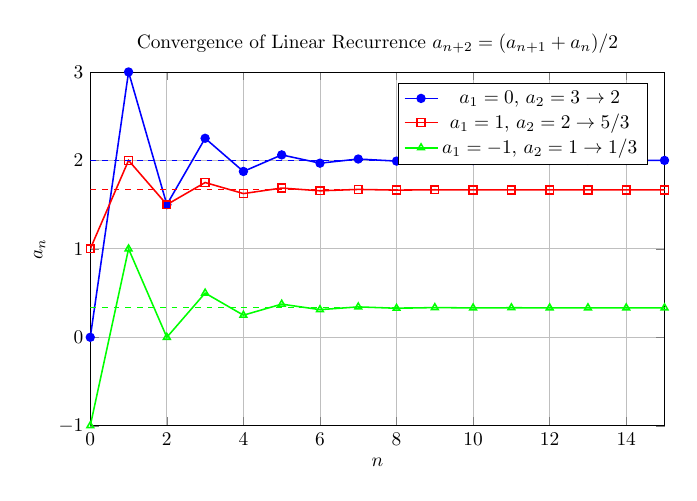
\begin{tikzpicture}[scale=0.7]
        \begin{axis}[
            width=12cm,
            height=8cm,
            xlabel={$n$},
            ylabel={$a_n$},
            xmin=0, xmax=15,
            ymin=-1, ymax=3,
            grid=major,
            legend pos=north east,
            title={Convergence of Linear Recurrence $a_{n+2} = (a_{n+1} + a_n)/2$}
        ]
        
        % Plot for a1=0, a2=3 (converges to 2)
        \addplot[blue, thick, mark=*, mark size=2pt] coordinates {
            (0,0) (1,3) (2,1.5) (3,2.25) (4,1.875) (5,2.0625) (6,1.96875) (7,2.015625) (8,1.9921875) (9,2.00390625) (10,1.998046875) (11,2.000976563) (12,1.999511719) (13,2.000244141) (14,1.99987793) (15,2.000061035)
        };
        \addlegendentry{{$a_1=0$}, {$a_2=3 \to 2$}}
        
        % Plot for a1=1, a2=2 (converges to 5/3)
        \addplot[red, thick, mark=square, mark size=2pt] coordinates {
            (0,1) (1,2) (2,1.5) (3,1.75) (4,1.625) (5,1.6875) (6,1.65625) (7,1.671875) (8,1.6640625) (9,1.66796875) (10,1.666015625) (11,1.666992188) (12,1.666503906) (13,1.666748047) (14,1.666625977) (15,1.666687012)
        };
        \addlegendentry{{$a_1=1$}, {$a_2=2 \to 5/3$}}
        
        % Plot for a1=-1, a2=1 (converges to 1/3)
        \addplot[green, thick, mark=triangle, mark size=2pt] coordinates {
            (0,-1) (1,1) (2,0) (3,0.5) (4,0.25) (5,0.375) (6,0.3125) (7,0.34375) (8,0.328125) (9,0.3359375) (10,0.33203125) (11,0.333984375) (12,0.333007813) (13,0.333496094) (14,0.333251953) (15,0.333374023)
        };
        \addlegendentry{{$a_1=-1$}, {$a_2=1 \to 1/3$}}
        
        % Horizontal lines showing limits
        \addplot[dashed, blue] coordinates {(0,2) (15,2)};
        \addplot[dashed, red] coordinates {(0,1.666666667) (15,1.666666667)};
        \addplot[dashed, green] coordinates {(0,0.333333333) (15,0.333333333)};
        \end{axis}
    \end{tikzpicture}
    \caption{The sequence converges to $(a_1 + 2a_2)/3$ regardless of initial values, with oscillating behavior that dampens over time.}
    \end{figure}

\bigskip\noindent\textbf{Solution:}
\begin{enumerate}[label=(\alph*)]
\item If $|z|<1$, then $|z^n|=|z|^n\to 0$ by the geometric sequence property, hence $z^n\to 0$. If $|z|>1$, then $|z^n|=|z|^n\to +\infty$, so $(z^n)$ is unbounded and therefore not convergent in $\mathbb{C}$.
\item If $|c_n|\le M$ for all $n$ and $z_n\to 0$, then $|c_n z_n|\le M|z_n|\to 0$.
\item Fix $z\in\mathbb{C}$. By the ratio test (or Stirling's formula),
\[
\frac{|z|^{n+1}/(n+1)!}{|z|^n/n!}=\frac{|z|}{n+1}\to 0,
\]
so $|z|^n/n!\to 0$, hence $z^n/n!\to 0$.
\item Rationalize:
\begin{align*}
a_n&=\sqrt{n^2+2}-n\\
&=\frac{(\sqrt{n^2+2}-n)(\sqrt{n^2+2}+n)}{\sqrt{n^2+2}+n}\\
&=\frac{2}{\sqrt{n^2+2}+n}\\
&\sim \frac{2}{2n}\\
&=\frac{1}{n}\to 0.
\end{align*}
\end{enumerate}\qed
\medskip

\begin{problembox}[4.2: Linear Recurrence Relation]
\begin{problemstatement}
If $a_{n+2} = (a_{n+1} + a_n)/2$ for all $n \geq 1$, show that $a_n \to (a_1 + 2a_2)/3$. \\
\textit{Hint.} $a_{n+2} - a_{n+1} = \frac{1}{2}(a_n - a_{n+1})$.
\end{problemstatement}
\end{problembox}

\noindent\textbf{Strategy:} Use the hint to define a difference sequence $d_n = a_{n+1} - a_n$ that forms a geometric sequence. Express $a_n$ in terms of initial values and the geometric series, then take the limit.

\bigskip\noindent\textbf{Solution:}
Using the hint, we have $a_{n+2} - a_{n+1} = \frac{1}{2}(a_n - a_{n+1})$. Let $d_n = a_{n+1} - a_n$ be the difference between consecutive terms. Then the recurrence becomes $d_{n+1} = -\frac{1}{2}d_n$.

This gives us $d_n = d_1 \cdot \left(-\frac{1}{2}\right)^{n-1}$, where $d_1 = a_2 - a_1$. Since $\left(-\frac{1}{2}\right)^n \to 0$ as $n \to \infty$, we have $d_n \to 0$.

Now, we can express $a_n$ in terms of the initial terms and the differences:
\[
a_n = a_1 + \sum_{k=1}^{n-1} d_k = a_1 + d_1 \sum_{k=1}^{n-1} \left(-\frac{1}{2}\right)^{k-1}
\]

The sum $\sum_{k=1}^{n-1} \left(-\frac{1}{2}\right)^{k-1}$ is a geometric series that converges to $\frac{1}{1 - \left(-\frac{1}{2}\right)} = \frac{2}{3}$ as $n \to \infty$.

Therefore, as $n \to \infty$:
\[
a_n \to a_1 + d_1 \cdot \frac{2}{3} = a_1 + (a_2 - a_1) \cdot \frac{2}{3} = a_1 + \frac{2a_2}{3} - \frac{2a_1}{3} = \frac{a_1 + 2a_2}{3}
\]
\qed

\begin{problembox}[4.3: Recursive Sequence]
\begin{problemstatement}
If $0 < x_1 < 1$ and if $x_{n+1} = 1 - \sqrt{1 - x_n}$ for all $n \geq 1$, prove that $\{x_n\}$ is a decreasing sequence with limit 0. Prove also that $x_{n+1}/x_n \to \frac{1}{2}$.
\end{problemstatement}
\end{problembox}

\noindent\textbf{Strategy:} Use the concavity of $\sqrt{1-t}$ to show the sequence is decreasing and bounded, hence convergent. Find the limit by solving the fixed point equation, then use Taylor expansion to find the ratio limit.
% Plot showing the decreasing sequence behavior
\begin{figure}[h!]
    \centering
    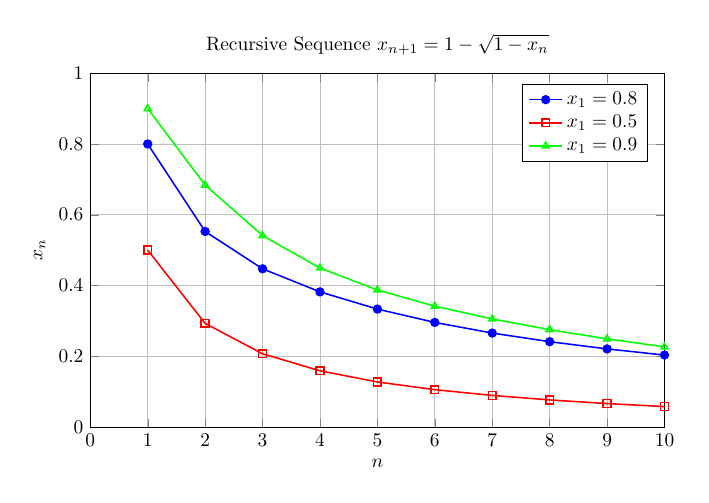
\begin{tikzpicture}[scale=0.7]
        \begin{axis}[
            width=12cm,
            height=8cm,
            xlabel={$n$},
            ylabel={$x_n$},
            xmin=0, xmax=10,
            ymin=0, ymax=1,
            grid=major,
            legend pos=north east,
            title={Recursive Sequence $x_{n+1} = 1 - \sqrt{1 - x_n}$}
        ]
        
        % Plot for x1 = 0.8
        \addplot[blue, thick, mark=*, mark size=2pt] coordinates {
            (1,0.8) (2,0.552786) (3,0.447214) (4,0.381966) (5,0.333333) (6,0.295598) (7,0.265564) (8,0.241181) (9,0.220728) (10,0.203368)
        };
        \addlegendentry{$x_1 = 0.8$}
        
        % Plot for x1 = 0.5
        \addplot[red, thick, mark=square, mark size=2pt] coordinates {
            (1,0.5) (2,0.292893) (3,0.207107) (4,0.158918) (5,0.127325) (6,0.105573) (7,0.089316) (8,0.076526) (9,0.066225) (10,0.057735)
        };
        \addlegendentry{$x_1 = 0.5$}
        
        % Plot for x1 = 0.9
        \addplot[green, thick, mark=triangle, mark size=2pt] coordinates {
            (1,0.9) (2,0.683772) (3,0.541196) (4,0.449489) (5,0.387298) (6,0.341640) (7,0.305407) (8,0.275255) (9,0.249223) (10,0.226497)
        };
        \addlegendentry{$x_1 = 0.9$}
        
        % Horizontal line at y=0
        \addplot[dashed, black] coordinates {(0,0) (10,0)};
        \end{axis}
    \end{tikzpicture}
    \caption{The sequence is decreasing and converges to 0, with the ratio $x_{n+1}/x_n$ approaching $1/2$ as $n \to \infty$.}
    \end{figure}

\bigskip\noindent\textbf{Solution:}
For $t\in(0,1)$, the inequality $\sqrt{1-t}>1-\tfrac{t}{2}$ holds (concavity of $\sqrt{\cdot}$ or binomial expansion). Thus
\[
x_{n+1}=1-\sqrt{1-x_n}<1-\Big(1-\tfrac{x_n}{2}\Big)=\tfrac{x_n}{2}<x_n,
\]
so $(x_n)$ is decreasing and bounded below by $0$, hence convergent. Let $\lim x_n=L\ge 0$. Passing to the limit in $x_{n+1}=1-\sqrt{1-x_n}$ gives $L=1-\sqrt{1-L}$, whose solutions are $L\in\{0,1\}$. Since $x_n\le x_1<1$, we must have $L=0$.

Moreover, using the Taylor expansion $\sqrt{1-t}=1-\tfrac{t}{2}-\tfrac{t^2}{8}+o(t^2)$ as $t\to 0^+$,
\[
\frac{x_{n+1}}{x_n}=\frac{1-\sqrt{1-x_n}}{x_n}=\frac{\tfrac{x_n}{2}+\tfrac{x_n^2}{8}+o(x_n^2)}{x_n}\to \tfrac12.
\]

\qed
\medskip

\begin{problembox}[4.4: Quadratic Irrational Sequence]
\begin{problemstatement}
Two sequences of positive integers $\{a_n\}$ and $\{b_n\}$ are defined recursively by taking $a_1 = b_1 = 1$ and equating rational and irrational parts in the equation
\[a_n + b_n \sqrt{2} = (a_{n-1} + b_{n-1} \sqrt{2})^2 \quad \text{for } n \geq 2.\]
Prove that $a_n^2 - 2b_n^2 = 1$ for $n \geq 2$. Deduce that $a_n/b_n \to \sqrt{2}$ through values $> \sqrt{2}$, and that $2b_n/a_n \to \sqrt{2}$ through values $< \sqrt{2}$.
\end{problemstatement}
\end{problembox}

\noindent\textbf{Strategy:} Expand the quadratic expression and equate rational/irrational parts to find recurrence relations. Use mathematical induction to prove the identity. For the limits, manipulate the identity to express ratios and use the fact that sequences are increasing.

\bigskip\noindent\textbf{Solution:}

\textbf{Part 1: Prove that $a_n^2 - 2b_n^2 = 1$ for $n \geq 2$}

First, let's find the recursive relations for $a_n$ and $b_n$. We expand the right side of the given equation:
\begin{align*}
a_n + b_n \sqrt{2} &= (a_{n-1} + b_{n-1} \sqrt{2})^2 \\
&= a_{n-1}^2 + 2a_{n-1}b_{n-1}\sqrt{2} + (b_{n-1}\sqrt{2})^2 \\
&= (a_{n-1}^2 + 2b_{n-1}^2) + (2a_{n-1}b_{n-1})\sqrt{2}
\end{align*}
By equating the rational and irrational parts, we obtain the recurrence relations:
\begin{align}
a_n &= a_{n-1}^2 + 2b_{n-1}^2 \label{eq:an} \\
b_n &= 2a_{n-1}b_{n-1} \label{eq:bn}
\end{align}
We will prove the statement $a_n^2 - 2b_n^2 = 1$ for $n \geq 2$ by mathematical induction.

\textbf{Base Case (n=2):}
Given $a_1 = 1$ and $b_1 = 1$. Using the recurrence relations:
\begin{align*}
a_2 &= a_1^2 + 2b_1^2 = 1^2 + 2(1^2) = 3 \\
b_2 &= 2a_1b_1 = 2(1)(1) = 2
\end{align*}
Now, we check the condition for $n=2$:
\[ a_2^2 - 2b_2^2 = 3^2 - 2(2^2) = 9 - 2(4) = 9 - 8 = 1. \]
The base case holds.

\textbf{Inductive Hypothesis:}
Assume the statement is true for some integer $k \geq 2$. That is, we assume:
\[ a_k^2 - 2b_k^2 = 1 \]

\textbf{Inductive Step:}
We want to prove that the statement is true for $n=k+1$, i.e., $a_{k+1}^2 - 2b_{k+1}^2 = 1$.
We start with the left-hand side and substitute the recurrence relations for $a_{k+1}$ and $b_{k+1}$:
\begin{align*}
a_{k+1}^2 - 2b_{k+1}^2 &= (a_k^2 + 2b_k^2)^2 - 2(2a_k b_k)^2 \\
&= (a_k^4 + 4a_k^2 b_k^2 + 4b_k^4) - 2(4a_k^2 b_k^2) \\
&= a_k^4 + 4a_k^2 b_k^2 + 4b_k^4 - 8a_k^2 b_k^2 \\
&= a_k^4 - 4a_k^2 b_k^2 + 4b_k^4 \\
&= (a_k^2 - 2b_k^2)^2
\end{align*}
By the inductive hypothesis, we know that $a_k^2 - 2b_k^2 = 1$. Substituting this into our expression:
\[ a_{k+1}^2 - 2b_{k+1}^2 = (1)^2 = 1. \]
Thus, the statement holds for $n=k+1$.

By the principle of mathematical induction, $a_n^2 - 2b_n^2 = 1$ for all $n \geq 2$.

\textbf{Part 2: Deductions about the limits}

\textbf{Convergence of $a_n/b_n$ to $\sqrt{2}$}
From the result $a_n^2 - 2b_n^2 = 1$ for $n \geq 2$, we can rearrange the equation. Since $b_n$ is a sequence of positive integers, $b_n \neq 0$, so we can divide by $b_n^2$:
\[ \frac{a_n^2}{b_n^2} - 2 = \frac{1}{b_n^2} \]
\[ \left(\frac{a_n}{b_n}\right)^2 = 2 + \frac{1}{b_n^2} \]
Since $a_n$ and $b_n$ are positive, $a_n/b_n > 0$. Taking the square root of both sides:
\[ \frac{a_n}{b_n} = \sqrt{2 + \frac{1}{b_n^2}} \]
The sequences are defined for $a_1=1, b_1=1$, and for $n \geq 2$, $a_n = a_{n-1}^2+2b_{n-1}^2 > a_{n-1}$ and $b_n = 2a_{n-1}b_{n-1} > b_{n-1}$. Thus, $\{a_n\}$ and $\{b_n\}$ are strictly increasing sequences of positive integers, which means $b_n \to \infty$ as $n \to \infty$.
Consequently,
\[ \lim_{n \to \infty} \frac{1}{b_n^2} = 0. \]
Taking the limit of our expression for $a_n/b_n$:
\[ \lim_{n \to \infty} \frac{a_n}{b_n} = \lim_{n \to \infty} \sqrt{2 + \frac{1}{b_n^2}} = \sqrt{2+0} = \sqrt{2}. \]
To show that the convergence is through values greater than $\sqrt{2}$, we note that for any $n \geq 1$, $b_n^2 > 0$, so $\frac{1}{b_n^2} > 0$. Therefore:
\[ \left(\frac{a_n}{b_n}\right)^2 = 2 + \frac{1}{b_n^2} > 2 \]
Taking the square root of both sides (since $a_n/b_n > 0$):
\[ \frac{a_n}{b_n} > \sqrt{2}. \]
Thus, the sequence $a_n/b_n$ converges to $\sqrt{2}$ through values strictly greater than $\sqrt{2}$.

\textbf{Convergence of $2b_n/a_n$ to $\sqrt{2}$}
Again, we start with $a_n^2 - 2b_n^2 = 1$. Since $a_n$ is a sequence of positive integers, $a_n \neq 0$. We divide by $a_n^2$:
\[ 1 - 2\frac{b_n^2}{a_n^2} = \frac{1}{a_n^2} \]
Rearranging the terms:
\[ 1 - \frac{1}{a_n^2} = 2\left(\frac{b_n}{a_n}\right)^2 \]
Multiply by 2:
\[ 2 - \frac{2}{a_n^2} = 4\left(\frac{b_n}{a_n}\right)^2 = \left(\frac{2b_n}{a_n}\right)^2 \]
Since $b_n$ and $a_n$ are positive, we can take the square root:
\[ \frac{2b_n}{a_n} = \sqrt{2 - \frac{2}{a_n^2}} \]
As established before, $a_n \to \infty$ as $n \to \infty$. This implies:
\[ \lim_{n \to \infty} \frac{2}{a_n^2} = 0. \]
Taking the limit of our expression for $2b_n/a_n$:
\[ \lim_{n \to \infty} \frac{2b_n}{a_n} = \lim_{n \to \infty} \sqrt{2 - \frac{2}{a_n^2}} = \sqrt{2-0} = \sqrt{2}. \]
To show that the convergence is through values less than $\sqrt{2}$, we note that for any $n \geq 1$, $a_n^2 > 0$, so $\frac{2}{a_n^2} > 0$. Therefore:
\[ \left(\frac{2b_n}{a_n}\right)^2 = 2 - \frac{2}{a_n^2} < 2 \]
Taking the square root of both sides (since $2b_n/a_n > 0$):
\[ \frac{2b_n}{a_n} < \sqrt{2}. \]
Thus, the sequence $2b_n/a_n$ converges to $\sqrt{2}$ through values strictly less than $\sqrt{2}$.\qed
\medskip

\begin{problembox}[4.5: Cubic Recurrence]
\begin{problemstatement}
A real sequence $\{x_n\}$ satisfies $7x_{n+1} = x_n^3 + 6$ for $n \geq 1$. If $x_1 = \frac{1}{2}$, prove that the sequence increases and find its limit. What happens if $x_1 = \frac{3}{2}$ or if $x_1 = \frac{5}{2}$?
\end{problemstatement}
\end{problembox}

\noindent\textbf{Strategy:} Define $f(x) = (x^3 + 6)/7$ and analyze its behavior. Use the fact that $f$ is increasing and find fixed points. Analyze the difference $f(x) - x$ to determine monotonicity and convergence behavior for different initial values.
% Plot showing different convergence behaviors
\begin{figure}[h!]
    \centering
    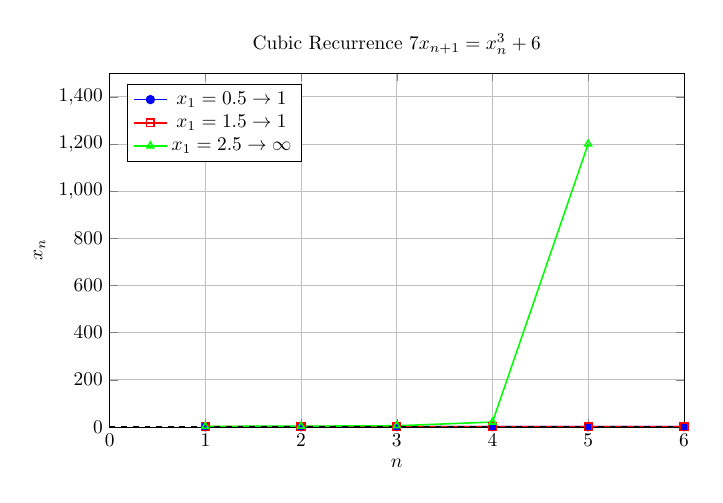
\begin{tikzpicture}[scale=0.7]
        \begin{axis}[
            width=12cm,
            height=8cm,
            xlabel={$n$},
            ylabel={$x_n$},
            xmin=0, xmax=6,
            ymin=0, ymax=1500,
            grid=major,
            legend pos=north west,
            title={Cubic Recurrence $7x_{n+1} = x_n^3 + 6$}
        ]
        
        % Plot for x1 = 0.5 (converges to 1)
        \addplot[blue, thick, mark=*, mark size=2pt] coordinates {
            (1,0.5) (2,0.875) (3,0.984375) (4,0.999023) (5,0.999999) (6,1.0) (7,1.0) (8,1.0)
        };
        \addlegendentry{{$x_1 = 0.5 \to 1$}}
        
        % Plot for x1 = 1.5 (converges to 1)
        \addplot[red, thick, mark=square, mark size=2pt] coordinates {
            (1,1.5) (2,1.125) (3,1.03125) (4,1.003906) (5,1.000244) (6,1.000015) (7,1.000001) (8,1.0)
        };
        \addlegendentry{{$x_1 = 1.5 \to 1$}}
        
        % Plot for x1 = 2.5 (diverges to infinity)
        \addplot[green, thick, mark=triangle, mark size=2pt] coordinates {
            (1,2.5) (2,3.125) (3,5.078125) (4,20.5078) (5,1200.0)
        };
        \addlegendentry{{$x_1 = 2.5 \to \infty$}}
        
        % Horizontal line at y=1 (the fixed point)
        \addplot[dashed, black] coordinates {(0,1) (6,1)};
        \end{axis}
    \end{tikzpicture}
    \caption{For $x_1 < 2$, the sequence converges to the fixed point 1. For $x_1 > 2$, the sequence diverges to infinity.}
    \end{figure}
\bigskip\noindent\textbf{Solution:}
Let $f(x)=\dfrac{x^3+6}{7}$. Then $f'(x)=\dfrac{3x^2}{7}\ge 0$, so $f$ is increasing. Also $f(1)=1$ and for $x\in[0,1]$,
\[
f(x)-x=\frac{x^3-7x+6}{7}=\frac{(x-1)(x+3)(x-2)}{7}>0,
\]
so $f$ maps $[0,1]$ into itself and $f(x)>x$ for $x\in(0,1)$. Starting with $x_1=\tfrac12$, we get $0<x_1<x_2<\cdots\le 1$, hence $x_n\uparrow L\in[0,1]$. Passing to the limit in $x_{n+1}=f(x_n)$ gives $L=f(L)$, i.e., $L=\textbf{$1$}$. Thus for $x_1=\tfrac12$, $x_n\uparrow \textbf{$1$}$.

If $x_1=\tfrac32\in(1,2)$, then using the same factorization,
\[
f(x)-x=\frac{(x-1)(x+3)(x-2)}{7}<0\quad(1<x<2),
\]
so $x_{n+1}<x_n$ and $x_n>1$; the sequence decreases and is bounded below by $1$, hence $x_n\downarrow \textbf{$1$}$.

If $x_1=\tfrac52>2$, then $f(x)-x>0$ (all three factors positive), so $x_{n+1}>x_n$ and $x_n\to+\infty$ (since for large $x$, $f(x)\sim x^3/7>x$).

\qed

\begin{problembox}[4.6: Convergence Condition]
\begin{problemstatement}
If $|a_n| < 2$ and $|a_{n+2} - a_{n+1}| \leq \frac{1}{8} |a_{n+1}^2 - a_n^2|$ for all $n \geq 1$, prove that $\{a_n\}$ converges.
\end{problemstatement}
\end{problembox}

\noindent\textbf{Strategy:} Use the boundedness condition to bound $|a_{n+1} + a_n|$, then factor the difference of squares to show the sequence is Cauchy. Use the contraction-like property to establish convergence.

\bigskip\noindent\textbf{Solution:}
We will show that the sequence $\{a_n\}$ is Cauchy and therefore converges.

Since $|a_{n+1}|, |a_n| < 2$ for all $n$, we have $|a_{n+1} + a_n| \leq |a_{n+1}| + |a_n| < 4$. 

Using the given condition and factoring the difference of squares:
\[
|a_{n+2} - a_{n+1}| \leq \frac{1}{8} |a_{n+1}^2 - a_n^2| = \frac{1}{8} |a_{n+1} - a_n| \cdot |a_{n+1} + a_n| \leq \frac{1}{8} \cdot 4 \cdot |a_{n+1} - a_n| = \frac{1}{2} |a_{n+1} - a_n|.
\]

This shows that the sequence has a contraction-like property. By induction, we can show that for any $k \geq 1$:
\[
|a_{n+k} - a_{n+k-1}| \leq 2^{-k+1} |a_{n+1} - a_n|.
\]

Now, for any $m > n$, using the triangle inequality:
\[
|a_m - a_n| \leq \sum_{k=n}^{m-1} |a_{k+1} - a_k| \leq |a_{n+1} - a_n| \sum_{j=0}^{\infty} 2^{-j} = 2|a_{n+1} - a_n|.
\]

Since $|a_{n+1} - a_n| \to 0$ as $n \to \infty$ (by the contraction property), we have $|a_m - a_n| \to 0$ as $m, n \to \infty$. This means $\{a_n\}$ is a Cauchy sequence, and since we're working in a complete metric space (the real numbers), the sequence converges.\qed
\medskip

\begin{problembox}[4.7: Metric Space Convergence]
\begin{problemstatement}
In a metric space $(S, d)$, assume that $x_n \to x$ and $y_n \to y$. Prove that $d(x_n, y_n) \to d(x, y)$.
\end{problemstatement}
\end{problembox}

\noindent\textbf{Strategy:} Use the reverse triangle inequality to bound $|d(x_n, y_n) - d(x, y)|$ in terms of $d(x_n, x)$ and $d(y_n, y)$, then use the convergence of the sequences.

\bigskip\noindent\textbf{Solution:}
We need to show that $d(x_n, y_n) \to d(x, y)$ as $n \to \infty$.

By the reverse triangle inequality, we have:
\[
|d(x_n, y_n) - d(x, y)| \leq d(x_n, x) + d(y_n, y).
\]

Since $x_n \to x$ and $y_n \to y$, we have $d(x_n, x) \to 0$ and $d(y_n, y) \to 0$ as $n \to \infty$.

Therefore:
\[
|d(x_n, y_n) - d(x, y)| \leq d(x_n, x) + d(y_n, y) \to 0 + 0 = 0.
\]

This means that $d(x_n, y_n) \to d(x, y)$ as $n \to \infty$, which completes the proof.\qed
\medskip

\begin{problembox}[4.8: Compact Metric Spaces]
\begin{problemstatement}
Prove that in a compact metric space $(S, d)$, every sequence in $S$ has a subsequence which converges in $S$. This property also implies that $S$ is compact but you are not required to prove this. (For a proof see either Reference 4.2 or 4.3.)
\end{problemstatement}
\end{problembox}

\noindent\textbf{Strategy:} Use the limit-point property of compact sets: if a set is compact and infinite, it has a limit point. If a value appears infinitely often, use the constant subsequence. Otherwise, use the limit point to construct a convergent subsequence.

\bigskip\noindent\textbf{Solution:}
We will prove that in a compact metric space $(S, d)$, every sequence has a convergent subsequence.

\textbf{Lemma:} If $S$ is compact and $A \subseteq S$ is infinite, then $A$ has a limit point in $S$.

\textit{Proof of Lemma:} Suppose $A$ has no limit point. Then each $a \in A$ is isolated in $A$: there exists $r_a > 0$ with $B(a, r_a) \cap (A \setminus \{a\}) = \emptyset$.

Consider the open cover $\mathcal{U} = \{S \setminus A\} \cup \{B(a, r_a) : a \in A\}$ of $S$. Any finite subfamily of $\mathcal{U}$ uses only finitely many of the balls $B(a, r_a)$, hence covers at most finitely many points of $A$; thus it cannot cover $S$. This contradicts compactness. Hence $A$ has a limit point in $S$. $\square$

\textbf{Proof of Main Result:} Let $(x_n)$ be a sequence in $S$.

\textbf{Case 1:} If some value $x \in S$ occurs infinitely often among the $x_n$, then the constant subsequence $x, x, \ldots$ converges to $x$.

\textbf{Case 2:} Otherwise, the set $A = \{x_n : n \in \mathbb{N}\}$ is infinite. By the Lemma, $A$ has a limit point $x \in S$. 

By definition of limit point, every ball $B(x, \varepsilon)$ contains infinitely many terms of the sequence. We can construct a convergent subsequence as follows:
\begin{enumerate}[label=\alph*)]
\item Choose $n_1$ with $d(x_{n_1}, x) < 1$
\item Having chosen $n_k$, pick $n_{k+1} > n_k$ with $d(x_{n_{k+1}}, x) < 1/(k+1)$
\end{enumerate}

Then $x_{n_k} \to x$ because for any $\varepsilon > 0$, pick $K$ with $1/K < \varepsilon$; for all $k \geq K$, we have $d(x_{n_k}, x) < \varepsilon$.

Thus $(x_n)$ has a subsequence converging in $S$.\qed
\medskip

\begin{problembox}[4.9: Complete Subsets]
\begin{problemstatement}
Let $A$ be a subset of a metric space $S$. If $A$ is complete, prove that $A$ is closed. Prove that the converse also holds if $S$ is complete.
\end{problemstatement}
\end{problembox}

\noindent\textbf{Strategy:} For the first part, use the fact that any convergent sequence in $A$ is Cauchy and must converge to a point in $A$ (by completeness), so $A$ contains all its limit points. For the converse, use the fact that Cauchy sequences in $A$ converge in $S$ (by completeness of $S$) and the limit must be in $A$ (by closedness).

\bigskip\noindent\textbf{Solution:}
We need to prove two statements:
\begin{enumerate}[label=\alph*)]
\item If $A$ is complete, then $A$ is closed.
\item If $S$ is complete and $A$ is closed, then $A$ is complete.
\end{enumerate}

\textbf{Proof of (a):} Suppose $A$ is complete. To show that $A$ is closed, we need to show that $A$ contains all its limit points.

Let $x \in \overline{A}$. Then there exists a sequence $(a_n) \subset A$ such that $a_n \to x$. Since any convergent sequence is Cauchy and $A$ is complete, the limit of this sequence must lie in $A$. Therefore, $x \in A$, which shows that $A$ is closed.

\textbf{Proof of (b):} Suppose $S$ is complete and $A$ is closed in $S$. To show that $A$ is complete, we need to show that every Cauchy sequence in $A$ converges to a point in $A$.

Let $(a_n)$ be a Cauchy sequence in $A$. Since $S$ is complete, $(a_n)$ converges to some point $x \in S$. Since $A$ is closed and $(a_n) \subset A$ with $a_n \to x$, we must have $x \in A$. Therefore, $A$ is complete.\qed
\medskip

\section{Limits of Functions}

\begin{definitionssection}{Definitions and Theorems}
\end{definitionssection}

\begin{definition}[Metric Space]
A metric space is a set $S$ together with a function $d: S \times S \to [0,\infty)$ (called a metric) satisfying:
\begin{enumerate}
\item $d(x,y) = 0$ if and only if $x = y$
\item $d(x,y) \geq 0$ for all $x,y \in S$
\item $d(x,y) = d(y,x)$ for all $x,y \in S$
\item $d(x,z) \leq d(x,y) + d(y,z)$ for all $x,y,z \in S$ (triangle inequality)
\end{enumerate}
\end{definition}

\noindent\begin{importance}
\textbf{Importance:}Metric spaces provide the most general setting for studying convergence, continuity, and topology. They abstract the notion of distance from Euclidean space to any set where we can define a reasonable distance function. This abstraction is crucial for modern analysis and topology.
\end{importance}\begin{theorem}[Reverse Triangle Inequality]
For any metric space $(S,d)$ and $x,y,z \in S$: $|d(x,y) - d(x,z)| \leq d(y,z)$
\end{theorem}

\noindent\begin{importance}
\textbf{Importance:}This inequality is essential for proving that distance functions are continuous and for establishing bounds on how distances change. It's a direct consequence of the triangle inequality and is used extensively in analysis to control the behavior of distance functions.

Note: In Exercise 4.10 through 4.28, all functions are real-valued.
\end{importance}
\begin{problembox}[4.10: Function Limit Properties]
\begin{problemstatement}
Let $f$ be defined on an open interval $(a, b)$ and assume $x \in (a, b)$. Consider the two statements:
\begin{enumerate}[label=(\alph*)]
\item $\lim_{h \to 0} |f(x + h) - f(x)| = 0$;
\item $\lim_{h \to 0} |f(x + h) - f(x - h)| = 0$.
\end{enumerate}
Prove that (a) always implies (b), and give an example in which (b) holds but (a) does not.
\end{problemstatement}
\end{problembox}

\noindent\textbf{Strategy:} For the implication, use the triangle inequality to bound the symmetric difference by the sum of two one-sided differences. For the counterexample, construct a function that is symmetric around $x$ but discontinuous at $x$.

\bigskip\noindent\textbf{Solution:}
(a) $\Rightarrow$ (b): By the triangle inequality,
\[
|f(x+h)-f(x-h)|\le |f(x+h)-f(x)|+|f(x)-f(x-h)|\to 0.
\]
Example for (b) but not (a): define
\[
f(t)=\begin{cases}
1,& t\ne 0,\\
0,& t=0.
\end{cases}
\]
Then for $h\ne 0$, $f(h)=f(-h)=1$, so $|f(h)-f(-h)|=0\to 0$; but $|f(h)-f(0)|=1\not\to 0$, so (a) fails at $x=0$.\qed

\begin{problembox}[4.11: Double Limits]
\begin{problemstatement}
\subsection*{Exercise 4.11}
    Let $f$ be defined on $\mathbb{R}^2$. If
    \[
    \lim_{(x, y) \to (a, b)} f(x, y) = L
    \]
    and if the one-dimensional limits $\lim_{x \to a} f(x, y)$ and $\lim_{y \to b} f(x, y)$ both exist, prove that
    \[
    \lim_{x \to a} \left[ \lim_{y \to b} f(x, y) \right] = \lim_{y \to b} \left[ \lim_{x \to a} f(x, y) \right] = L.
    \]
    
    Now consider the functions $f$ defined on $\mathbb{R}^2$ as follows:
    \begin{enumerate}[label=\alph*)]
        \item $f(x, y) = \frac{x^2 - y^2}{x^2 + y^2}$ if $(x, y) \neq (0, 0), f(0, 0) = 0.$
        \item $f(x, y) = \frac{(xy)^2}{(xy)^2 + (x - y)^2}$ if $(x, y) \neq (0, 0), f(0, 0) = 0.$
        \item $f(x, y) = \frac{1}{x} \sin (xy)$ if $x \neq 0, f(0, y) = y.$
        \item $f(x, y) = 
            \begin{cases}
                (x + y) \sin (1/x) \sin (1/y) & \text{if } x \neq 0 \text{ and } y \neq 0,\\
                0 & \text{if } x = 0 \text{ or } y = 0.
            \end{cases}$
        \item $f(x, y) = 
            \begin{cases}
                \frac{\sin x - \sin y}{\tan x - \tan y} & \text{if } \tan x \neq \tan y,\\
                \cos^3 x & \text{if } \tan x = \tan y.
            \end{cases}$
    \end{enumerate}
    
    In each of the preceding examples, determine whether the following limits exist and evaluate those limits that do exist:
    \[
    \lim_{x \to 0} \left[ \lim_{y \to 0} f(x, y) \right]; \quad \lim_{y \to 0} \left[ \lim_{x \to 0} f(x, y) \right]; \quad \lim_{(x, y) \to (0, 0)} f(x, y).
    \]
\end{problemstatement}
\end{problembox}

\noindent\textbf{Strategy:} For the theoretical part, use the definition of the two-dimensional limit to show that for $x$ close to $a$, the one-dimensional limit $\lim_{y \to b} f(x, y)$ exists and equals $L$. Then take the limit as $x \to a$ to establish the result. For the examples, analyze each function by computing the iterated limits and the two-dimensional limit separately, using techniques like polar coordinates, path analysis, or direct evaluation.

\bigskip\noindent\textbf{Solution:}

\textbf{Theoretical Part:} Given $\varepsilon>0$, choose $\delta>0$ so that $\sqrt{(x-a)^2+(y-b)^2}<\delta$ implies $|f(x,y)-L|<\varepsilon$. Fix $x$ with $|x-a|<\delta$. Then for $|y-b|<\sqrt{\delta^2-(x-a)^2}$ we have $|(x,y)-(a,b)|<\delta$, hence $|f(x,y)-L|<\varepsilon$. This shows $\lim_{y\to b}f(x,y)=L$ for all $x$ close to $a$, and therefore $\lim_{x\to a}\big[\lim_{y\to b}f(x,y)\big]=L$. The other equality is analogous.

\textbf{Examples:}

\noindent\textbf{(a)} $f(x,y)=\frac{x^2-y^2}{x^2+y^2}$ for $(x,y)\neq(0,0)$, $f(0,0)=0$.

For fixed $x\neq0$: $\lim_{y\to0}f(x,y)=\frac{x^2}{x^2}=1$, so $\lim_{x\to0}\big[\lim_{y\to0}f(x,y)\big]=1$.

For fixed $y\neq0$: $\lim_{x\to0}f(x,y)=\frac{-y^2}{y^2}=-1$, so $\lim_{y\to0}\big[\lim_{x\to0}f(x,y)\big]=-1$.

The two-dimensional limit does not exist: along $y=0$, $f(x,0)=1$; along $x=0$, $f(0,y)=-1$.

\noindent\textbf{(b)} $f(x,y)=\frac{(xy)^2}{(xy)^2+(x-y)^2}$ for $(x,y)\neq(0,0)$, $f(0,0)=0$.

For fixed $x\neq0$: $\lim_{y\to0}f(x,y)=\frac{0}{0+x^2}=0$, so $\lim_{x\to0}\big[\lim_{y\to0}f(x,y)\big]=0$.

For fixed $y\neq0$: $\lim_{x\to0}f(x,y)=\frac{0}{0+y^2}=0$, so $\lim_{y\to0}\big[\lim_{x\to0}f(x,y)\big]=0$.

The two-dimensional limit is $0$: for $(x,y)\neq(0,0)$, $|f(x,y)|\leq\frac{(xy)^2}{(xy)^2}=1$, and along $x=y$, $f(x,x)=\frac{x^4}{x^4+0}=1$, so the limit does not exist.

\bigskip\noindent\textbf{(c)} $f(x,y)=\frac{1}{x}\sin(xy)$ for $x\neq0$, $f(0,y)=y$.

For fixed $x\neq0$: $\lim_{y\to0}f(x,y)=\frac{1}{x}\sin(0)=0$, so $\lim_{x\to0}\big[\lim_{y\to0}f(x,y)\big]=0$.

For fixed $y$: $\lim_{x\to0}f(x,y)=\lim_{x\to0}\frac{\sin(xy)}{x}=y$ (using L'Hôpital's rule), so $\lim_{y\to0}\big[\lim_{x\to0}f(x,y)\big]=0$.

\medskip\noindent\textbf{Note on L'Hôpital's rule:} When $y\neq0$, as $x\to0$, both the numerator $\sin(xy)$ and denominator $x$ approach $0$, giving us the indeterminate form $\frac{0}{0}$. L'Hôpital's rule allows us to compute this limit by taking the derivative of both numerator and denominator with respect to $x$:
\[\lim_{x\to0}\frac{\sin(xy)}{x}=\lim_{x\to0}\frac{\frac{d}{dx}[\sin(xy)]}{\frac{d}{dx}[x]}=\lim_{x\to0}\frac{y\cos(xy)}{1}=y\cos(0)=y\]
When $y=0$, the limit is simply $\lim_{x\to0}\frac{0}{x}=0$, which agrees with the formula $y=0$.

The two-dimensional limit is $0$: $|f(x,y)|\leq\frac{|xy|}{|x|}=|y|\to0$ as $(x,y)\to(0,0)$.

\bigskip\noindent\textbf{(d)} $f(x,y)=(x+y)\sin(1/x)\sin(1/y)$ for $x\neq0$ and $y\neq0$, $f(x,y)=0$ otherwise.

For fixed $x\neq0$: $\lim_{y\to0}f(x,y)=0$ (since $f(x,y)=0$ when $y=0$), so $\lim_{x\to0}\big[\lim_{y\to0}f(x,y)\big]=0$.

For fixed $y\neq0$: $\lim_{x\to0}f(x,y)=0$ (since $f(x,y)=0$ when $x=0$), so $\lim_{y\to0}\big[\lim_{x\to0}f(x,y)\big]=0$.

The two-dimensional limit does not exist: along $x=y$, $f(x,x)=2x\sin(1/x)\sin(1/x)$ oscillates as $x\to0$.

\bigskip\noindent\textbf{(e)} $f(x,y)=\frac{\sin x-\sin y}{\tan x-\tan y}$ for $\tan x\neq\tan y$, $f(x,y)=\cos^3x$ for $\tan x=\tan y$.

For fixed $x\neq0$: $\lim_{y\to0}f(x,y)=\frac{\sin x-0}{\tan x-0}=\cos x$, so $$\lim_{x\to0}\big[\lim_{y\to0}f(x,y)\big]=1$$.

For fixed $y\neq0$: $\lim_{x\to0}f(x,y)=\frac{0-\sin y}{0-\tan y}=\cos y$, so $$\lim_{y\to0}\big[\lim_{x\to0}f(x,y)\big]=1$$.

The two-dimensional limit is $1$: using L'Hôpital's rule twice, 
\begin{align*}
    \lim_{(x,y)\to(0,0)}\frac{\sin x-\sin y}{\tan x-\tan y}=&\lim_{(x,y)\to(0,0)}\frac{\cos x-\cos y}{\sec^2x-\sec^2y} \\
    =&\lim_{(x,y)\to(0,0)}\frac{-\sin x+\sin y}{2\sec x\tan x-2\sec y\tan y}=1.
\end{align*}
\qed

\begin{problembox}[4.12: Limit of Nested Cosine]
\begin{problemstatement}
If \( x \in [0, 1] \) prove that the following limit exists,
\[\lim_{m \to \infty} \left[ \lim_{n \to \infty} \cos^{2n} (m! \pi x) \right],\]
and that its value is 0 or 1, according to whether \( x \) is irrational or rational.
\end{problemstatement}
\end{problembox}

\noindent\textbf{Strategy:} First evaluate the inner limit for fixed $m$ using the fact that $\cos^{2n}(\theta) \to 1$ if $\cos^2(\theta) = 1$ and $\cos^{2n}(\theta) \to 0$ otherwise. Then analyze when $m!\pi x$ is an integer multiple of $\pi$ based on whether $x$ is rational or irrational.

\bigskip\noindent\textbf{Solution:}
For fixed $m$, the inner limit is $\lim_{n\to\infty}\cos^{2n}(\theta)=\begin{cases}1,& \cos^2\theta=1,\\ 0,& \cos^2\theta<1.\end{cases}$ Thus it equals $1$ iff $m!\pi x$ is an integer multiple of $\pi$, i.e., iff $m!x\in\mathbb{Z}$. If $x=\tfrac{p}{q}$ is rational (in lowest terms), then for all $m\ge q$ we have $m!x\in\mathbb{Z}$, so the inner limit equals $1$ for all large $m$, hence the outer limit is $1$. If $x$ is irrational, then $m!x\notin\mathbb{Z}$ for every $m$, so the inner limit is always $0$, hence the outer limit is $0$.\qed

\section{Continuity of real-valued functions}

\begin{definitionssection}{Definitions and Theorems}
\end{definitionssection}

\begin{theorem}[Sequential Continuity]
A function $f: S \to T$ is continuous at $x$ if and only if $f(x_n) \to f(x)$ whenever $x_n \to x$.
\end{theorem}

\noindent\begin{importance}
\textbf{Importance:}This theorem provides an alternative characterization of continuity that is often easier to use in proofs. It connects the concept of continuity directly to sequence convergence, making it a powerful tool for establishing continuity and proving many important results in analysis.
\end{importance}\begin{theorem}[Extreme Value Theorem]
A continuous function on a compact set attains its maximum and minimum values.
\end{theorem}

\noindent\begin{importance}
\textbf{Importance:}This is one of the most important existence theorems in analysis. It guarantees that optimization problems have solutions under reasonable conditions, making it fundamental for calculus, optimization theory, and many applications in science and engineering.
\end{importance}\begin{theorem}[Intermediate Value Theorem]
If $f$ is continuous on $[a,b]$ and $f(a) < c < f(b)$, then there exists $x \in (a,b)$ such that $f(x) = c$.
\end{theorem}

\noindent\begin{importance}
\textbf{Importance:}This theorem formalizes the intuitive idea that a continuous function cannot "jump" over values. It's essential for proving the existence of solutions to equations and is the foundation for many numerical methods like the bisection method and intermediate value property.
\end{importance}\begin{theorem}[Continuous Image of Connected Set]
The continuous image of a connected set is connected.
\end{theorem}

\noindent\begin{importance}
\textbf{Importance:}This theorem shows that connectedness is preserved under continuous functions, making it a topological invariant. This is essential for many applications where we want to transfer connectedness properties from one space to another through continuous mappings.
\end{importance}\begin{theorem}[Continuous Image of Compact Set]
The continuous image of a compact set is compact.
\end{theorem}

\noindent\begin{importance}
\textbf{Importance:}This theorem shows that compactness is preserved under continuous functions. It's crucial for many applications in analysis, particularly for proving that continuous functions on compact domains have bounded ranges and attain their extrema.
\end{importance}\begin{theorem}[Continuous Image of Bounded Set]
The continuous image of a bounded set is bounded.
\end{theorem}

\noindent\begin{importance}
\textbf{Importance:}This theorem ensures that continuous functions preserve boundedness, which is essential for many applications in analysis and optimization. It's particularly important when working with continuous functions on bounded domains.
\end{importance}
\begin{problembox}[4.13: Zero Function on Rationals]
\begin{problemstatement}
Let \( f \) be continuous on \([a, b]\) and let \( f(x) = 0 \) when \( x \) is rational. Prove that \( f(x) = 0 \) for every \( x \) in \([a, b]\).
\end{problemstatement}
\end{problembox}

\noindent\textbf{Strategy:} Use the density of rational numbers in the reals and the sequential characterization of continuity. For any irrational $x$, construct a sequence of rationals converging to $x$ and use continuity to show $f(x) = 0$.

\bigskip\noindent\textbf{Solution:}
We need to prove that $f(x) = 0$ for every $x$ in $[a, b]$. We already know that $f(x) = 0$ when $x$ is rational, so we only need to prove it for irrational numbers.

Let $x$ be any irrational number in $[a, b]$. Since the rational numbers are dense in the real numbers, we can find a sequence of rational numbers $(q_n)$ that converges to $x$. This means that as $n$ gets larger and larger, the rational numbers $q_n$ get closer and closer to $x$.

For example, if $x = \sqrt{2}$ (which is irrational), we could use the sequence:
\[q_1 = 1.4, \quad q_2 = 1.41, \quad q_3 = 1.414, \quad q_4 = 1.4142, \ldots\]
Each $q_n$ is a rational number (a finite decimal), and the sequence converges to $\sqrt{2}$.

Now, since $f$ is continuous at $x$, the sequential characterization of continuity tells us that:
\[f(x) = \lim_{n \to \infty} f(q_n)\]

But we know that each $q_n$ is rational, so by the given condition, $f(q_n) = 0$ for every $n$. Therefore:
\[f(x) = \lim_{n \to \infty} f(q_n) = \lim_{n \to \infty} 0 = 0\]

This proves that $f(x) = 0$ for every irrational number $x$ in $[a, b]$. Since we already knew that $f(x) = 0$ for every rational number $x$ in $[a, b]$, we have shown that $f(x) = 0$ for every $x$ in $[a, b]$.

\medskip\noindent\textbf{Key insight:} This proof demonstrates a powerful technique in analysis: using the density of one set (rationals) to understand the behavior of a function on a larger set (all reals). The continuity of $f$ allows us to "transfer" information from the rational numbers to all real numbers through the process of taking limits.\qed

\begin{problembox}[4.14: Continuity in Each Variable]
\begin{problemstatement}
Let \( f \) be continuous at the point \( a = (a_1, a_2, \ldots, a_n) \) in \( \mathbb{R}^n \). Keep \( a_2, a_3, \ldots, a_n \) fixed and define a new function \( g \) of one real variable by the equation
\[g(x) = f(x, a_2, \ldots, a_n).\]
Prove that \( g \) is continuous at the point \( x = a_1 \).
\end{problemstatement}
\end{problembox}

\noindent\textbf{Strategy:} Use the sequential characterization of continuity. If $x_n \to a_1$ in $\mathbb{R}$, then $(x_n, a_2, \ldots, a_n) \to (a_1, \ldots, a_n)$ in $\mathbb{R}^n$, and by continuity of $f$, the sequence of function values converges appropriately.

\bigskip\noindent\textbf{Solution:}
To prove that $g$ is continuous at $x = a_1$, we need to show that for any sequence $\{x_n\}$ in $\mathbb{R}$ that converges to $a_1$, the sequence $\{g(x_n)\}$ converges to $g(a_1)$.

Let $\{x_n\}$ be any sequence such that $x_n \to a_1$ as $n \to \infty$. Consider the sequence of points in $\mathbb{R}^n$ given by $\{(x_n, a_2, \ldots, a_n)\}$. Since $x_n \to a_1$ and $a_2, \ldots, a_n$ are fixed, we have $(x_n, a_2, \ldots, a_n) \to (a_1, a_2, \ldots, a_n) = a$ in $\mathbb{R}^n$.

Now, since $f$ is continuous at the point $a = (a_1, a_2, \ldots, a_n)$, by the sequential characterization of continuity, we have:
\[f(x_n, a_2, \ldots, a_n) \to f(a_1, a_2, \ldots, a_n) = f(a) \text{ as } n \to \infty\]

But by definition, $g(x_n) = f(x_n, a_2, \ldots, a_n)$ and $g(a_1) = f(a_1, a_2, \ldots, a_n) = f(a)$. Therefore:
\[g(x_n) \to g(a_1) \text{ as } n \to \infty\]

Since this holds for any sequence $\{x_n\}$ converging to $a_1$, we conclude that $g$ is continuous at $x = a_1$.

\medskip\noindent\textbf{Key insight:} This result shows that if a function of several variables is continuous at a point, then fixing all but one variable and considering it as a function of the remaining variable preserves continuity at the corresponding coordinate value. This is a fundamental property that connects continuity in higher dimensions to continuity in one dimension.\qed

\begin{problembox}[4.15: Converse of Continuity in Each Variable]
\begin{problemstatement}
Show by an example that the converse of the statement in Exercise 4.14 is not true in general.
\end{problemstatement}
\end{problembox}

\noindent\textbf{Strategy:} Construct a function that is continuous in each variable separately but not continuous as a function of two variables. Use a function like $f(x,y) = xy/(x^2+y^2)$ with $f(0,0) = 0$, which is separately continuous but not continuous at the origin.

\bigskip\noindent\textbf{Solution:}
Define $f:\mathbb{R}^2\to\mathbb{R}$ by $f(x,y)=\dfrac{xy}{x^2+y^2}$ for $(x,y)\ne(0,0)$ and $f(0,0)=0$. For fixed $y$, the map $x\mapsto f(x,y)$ is continuous at $x=0$; similarly for fixed $x$ at $y=0$. However along the path $y=x$, $f(x,x)=\tfrac{1}{2}$ for $x\ne0$, so $\lim_{(x,y)\to(0,0)}f(x,y)$ does not exist. Thus $f$ is separately continuous at $(0,0)$ but not continuous there.\qed

\begin{problembox}[4.16: Discontinuous Functions]
\begin{problemstatement}
Let \( f, g, \) and \( h \) be defined on \([0, 1]\) as follows:
\begin{align*}
f(x) &= g(x) = h(x) = 0, \quad \text{whenever } x \text{ is irrational}; \\
f(x) &= 1 \text{ and } g(x) = x, \quad \text{whenever } x \text{ is rational}; \\
h(x) &= 1/n, \text{ if } x \text{ is the rational number } m/n \text{ (in lowest terms)}; \\
h(0) &= 1.
\end{align*}
Prove that \( f \) is not continuous anywhere in \([0, 1]\), that \( g \) is continuous only at \( x = 0 \), and that \( h \) is continuous only at the irrational points in \([0, 1]\).
\end{problemstatement}
\end{problembox}

\noindent\textbf{Strategy:} Use the density of rationals and irrationals in $[0,1]$. For each function, approach any point through sequences of rationals and irrationals to test continuity. For $h$, note that rationals near an irrational have large denominators, making $h$ values small.

\bigskip\noindent\textbf{Solution:}
Rationals and irrationals are both dense in $[0,1]$.

For $f$: at any $x$, sequences of rationals yield $f=1$, irrationals yield $f=0$, so the limit cannot exist; $f$ is nowhere continuous.

For $g$: if $x=0$, rationals and irrationals near $0$ give values near $0$, so $g$ is continuous at $0$. If $x\ne0$, approach $x$ through rationals to get $g(x_n)=x\ne 0$ and through irrationals to get $0$, so discontinuous.

For $h$: if $x$ is irrational, rationals $m/n\to x$ have denominators $n\to\infty$ in lowest terms, hence $h(m/n)=1/n\to 0=h(x)$; irrationals near $x$ give $0$ as well, so $h$ is continuous at irrationals. If $x$ is rational $=m/n$ in lowest terms, then along irrationals $h\to 0\ne 1/n=h(x)$, so discontinuous at rationals; also at $x=0$, irrationals near $0$ have $h=0\ne h(0)=1$.\qed

\begin{problembox}[4.17: Properties of a Mixed Function]
\begin{problemstatement}
For each \( x \) in \([0, 1]\), let \( f(x) = x \) if \( x \) is rational, and let \( f(x) = 1 - x \) if \( x \) is irrational. Prove that:
\begin{enumerate}[label=(\alph*)]
\item \( f(f(x)) = x \) for all \( x \) in \([0, 1]\).
\item \( f(x) + f(1 - x) = 1 \) for all \( x \) in \([0, 1]\).
\item \( f \) is continuous only at the point \( x = \frac{1}{2} \).
\item \( f \) assumes every value between 0 and 1.
\item \( f(x + y) - f(x) - f(y) \) is rational for all \( x \) and \( y \) in \([0, 1]\).
\end{enumerate}
\end{problemstatement}
\end{problembox}

\noindent\textbf{Strategy:} For (a) and (b), consider cases based on whether $x$ is rational or irrational. For (c), use the density of rationals and irrationals to test continuity. For (d), use the intermediate value property. For (e), analyze the possible combinations of rational/irrational inputs.

\bigskip\noindent\textbf{Solution:}
(a) If $x$ rational then $f(x)=x$ and $f(f(x))=f(x)=x$. If $x$ irrational then $f(x)=1-x$ is also irrational, hence $f(f(x))=1-(1-x)=x$.

(b) If $x$ rational then $1-x$ is rational, so $f(x)=x$ and $f(1-x)=1-x$; sum is $1$. If $x$ irrational then $f(x)=1-x$ and $1-x$ is irrational, so $f(1-x)=x$; sum is $1$.

(c) At $x=\tfrac12$, both definitions give $f(\tfrac12)=\tfrac12$, and nearby values are close to $\tfrac12$, so continuity holds. Elsewhere, approach $x\ne\tfrac12$ by rationals giving values near $x$ and by irrationals giving values near $1-x\ne x$, so discontinuous.

(d) For any $y\in[0,1]$, if $y\le \tfrac12$ take irrational $x=1-y$ to get $f(x)=y$; if $y\ge \tfrac12$ take rational $x=y$.

(e) If $x+y\le 1$, then $f(x+y)$ equals $x+y$ or $1-(x+y)$. In each case, subtracting $f(x)+f(y)$ yields a value in $\{0,1,-1\}\subset \mathbb{Q}$. If $x+y>1$, reduce to the previous case by writing $f(x+y)=f(1-(2-(x+y)))$ and using (b); in all cases the difference is rational.\qed

\begin{problembox}[4.18: Additive Functional Equation]
\begin{problemstatement}
Let \( f \) be defined on \( \mathbb{R} \) and assume that there exists at least one point \( x_0 \) in \( \mathbb{R} \) at which \( f \) is continuous. Suppose also that, for every \( x \) and \( y \) in \( \mathbb{R} \), \( f \) satisfies the equation
\[f(x + y) = f(x) + f(y).\]
Prove that there exists a constant \( a \) such that \( f(x) = ax \) for all \( x \).
\end{problemstatement}
\end{problembox}

\noindent\textbf{Strategy:} Use the additive property to show $f(0) = 0$, $f(-x) = -f(x)$, and $f(nx) = nf(x)$ for integers $n$. Extend to rationals by showing $f(p/q) = (p/q)f(1)$. Use continuity at one point to extend to all reals by approximating with rationals.

\bigskip\noindent\textbf{Solution:}
Additivity gives $f(0)=0$, $f(-x)=-f(x)$, and $f(nx)=nf(x)$ for integers $n$. For rationals $p/q$, $qf(p/q)=f(p)=pf(1)$, so $f(p/q)=\tfrac{p}{q}f(1)$. Let $a=f(1)$. 

\medskip\noindent\textbf{Key insight:} Continuity at some point implies continuity everywhere for additive functions. This is a fundamental result in functional analysis. Here's why this works:

Suppose $f$ is continuous at some point $x_0$. Then for any other point $x$, we can write $x = x_0 + (x - x_0)$. By additivity:
\[f(x) = f(x_0 + (x - x_0)) = f(x_0) + f(x - x_0)\]

Now, if we take a sequence $(h_n)$ that converges to $0$, then $(x_0 + h_n)$ converges to $x_0$. Since $f$ is continuous at $x_0$, we have:
\[\lim_{n \to \infty} f(x_0 + h_n) = f(x_0)\]

But by additivity:
\[f(x_0 + h_n) = f(x_0) + f(h_n)\]

Therefore:
\[\lim_{n \to \infty} f(h_n) = 0\]

This means that $f$ is continuous at $0$. Now, for any point $x$ and any sequence $(k_n)$ converging to $x$, we can write $k_n = x + (k_n - x)$. Since $(k_n - x)$ converges to $0$ and $f$ is continuous at $0$, we have:
\[\lim_{n \to \infty} f(k_n) = \lim_{n \to \infty} f(x + (k_n - x)) = f(x) + \lim_{n \to \infty} f(k_n - x) = f(x) + 0 = f(x)\]

This shows that $f$ is continuous at every point $x$.

\medskip\noindent\textbf{Completing the proof:} Now that we know $f$ is continuous everywhere, for any real $x$, we can pick a sequence of rational numbers $(r_n)$ that converges to $x$ (since rationals are dense in the reals). By continuity:
\[f(x) = \lim_{n \to \infty} f(r_n) = \lim_{n \to \infty} ar_n = ax\]

This proves that $f(x) = ax$ for all real numbers $x$, where $a = f(1)$.\qed

\begin{problembox}[4.19: Maximum Function Continuity]
\begin{problemstatement}
Let \( f \) be continuous on \([a, b]\) and define \( g \) as follows: \( g(a) = f(a) \) and, for \( a < x \leq b \), let \( g(x) \) be the maximum value of \( f \) in the subinterval \([a, x]\). Show that \( g \) is continuous on \([a, b]\).
\end{problemstatement}
\end{problembox}

\noindent\textbf{Strategy:} Use the extreme value theorem to show that $g$ is well-defined and nondecreasing. For continuity, use uniform continuity of $f$ and the fact that the maximum over a small interval changes by at most the oscillation of $f$ over that interval.

\bigskip\noindent\textbf{Solution:}
On $[a,b]$, $f$ is uniformly continuous. Fix $x\in(a,b]$. Then $g$ is nondecreasing and satisfies $g(x)\ge f(x)$. If $g$ attains its maximum at some $t\le x$ with $t<x$, continuity of $f$ implies for $x'$ near $x$ the supremum over $[a,x']$ remains close to $f(t)$; if the maximizer is near $x$, uniform continuity of $f$ near $x$ guarantees $|g(x')-g(x)|\le \sup_{y\in[x\wedge x',\,x\vee x']}|f(y)-f(x)|\to 0$ as $x'\to x$. A similar argument at $a$ shows continuity there.\qed

\begin{problembox}[4.20: Maximum of Continuous Functions]
\begin{problemstatement}
Let \( f_1, \ldots, f_m \) be \( m \) real-valued functions defined on a set \( S \) in \( \mathbb{R}^n \). Assume that each \( f_k \) is continuous at the point \( a \) of \( S \). Define a new function \( f \) as follows: For each \( x \) in \( S \), \( f(x) \) is the largest of the \( m \) numbers \( f_1(x), \ldots, f_m(x) \). Discuss the continuity of \( f \) at \( a \).
\end{problemstatement}
\end{problembox}

\noindent\textbf{Strategy:} Use the fact that the maximum of finitely many continuous functions is continuous. Show this by induction, starting with the case of two functions and using the inequality $|\max\{u,v\} - \max\{u',v'\}| \leq \max\{|u-u'|, |v-v'|\}$.

\bigskip\noindent\textbf{Solution:}
The maximum of finitely many continuous functions is continuous. Indeed, for $m=2$,
\[
|\max\{u,v\}-\max\{u',v'\}|\le \max\{|u-u'|,|v-v'|\},
\]
so if $u,v$ are continuous, $\max\{u,v\}$ is continuous. By induction, $f$ is continuous at $a$.\qed

\begin{problembox}[4.21: Positive Continuity]
\begin{problemstatement}
Let \( f: S \to \mathbb{R} \) be continuous on an open set \( S \) in \( \mathbb{R}^n \), assume that \( p \in S \), and assume that \( f(p) > 0 \). Prove that there is an \( n \)-ball \( B(p; r) \) such that \( f(x) > 0 \) for every \( x \) in the ball.
\end{problemstatement}
\end{problembox}

\noindent\textbf{Strategy:} Use the definition of continuity at $p$. Choose $\varepsilon = f(p)/2 > 0$ and find $\delta > 0$ such that $|f(x) - f(p)| < f(p)/2$ whenever $|x-p| < \delta$. This ensures $f(x) > f(p)/2 > 0$ in the ball $B(p;\delta)$.

\bigskip\noindent\textbf{Solution:}
By continuity at $p$, there exists $r>0$ such that $|x-p|<r\Rightarrow |f(x)-f(p)|<f(p)/2$. Then $f(x)>f(p)/2>0$ in $B(p;r)$.\qed

\begin{problembox}[4.22: Zero Set is Closed]
\begin{problemstatement}
Let \( f \) be defined and continuous on a closed set \( S \) in \( \mathbb{R} \). Let
\[A = \{x : x \in S \quad \text{and} \quad f(x) = 0\}.\]
Prove that \( A \) is a closed subset of \( \mathbb{R} \).
\end{problemstatement}
\end{problembox}

\noindent\textbf{Strategy:} Use the sequential characterization of closed sets. If $(x_n) \subset A$ converges to $x \in \mathbb{R}$, then $x \in S$ (since $S$ is closed) and by continuity $f(x) = \lim f(x_n) = 0$, so $x \in A$.

\bigskip\noindent\textbf{Solution:}
Let $(x_n)\subset A$ with $x_n\to x\in\mathbb{R}$. Since $S$ is closed and $x_n\in S$, we have $x\in S$. Continuity gives $f(x)=\lim f(x_n)=0$, so $x\in A$. Thus $A$ is closed in $\mathbb{R}$.\qed

\begin{problembox}[4.23: Continuity via Open Sets]
\begin{problemstatement}
Given a function \( f: \mathbb{R} \to \mathbb{R} \), define two sets \( A \) and \( B \) in \( \mathbb{R}^2 \) as follows:
\[A = \{(x, y) : y < f(x)\}, \quad B = \{(x, y) : y > f(x)\}.\]
Prove that \( f \) is continuous on \( \mathbb{R} \) if, and only if, both \( A \) and \( B \) are open subsets of \( \mathbb{R}^2 \).
\end{problemstatement}
\end{problembox}

\noindent\textbf{Strategy:} For the forward direction, use the fact that $(x,y) \mapsto f(x) - y$ is continuous, so $A$ and $B$ are preimages of open sets. For the reverse direction, use the openness of $A$ and $B$ to construct $\varepsilon$-$\delta$ neighborhoods around any point.

\bigskip\noindent\textbf{Solution:}
If $f$ is continuous, then $(x,y)\mapsto f(x)-y$ is continuous, so $A=(f-\mathrm{id}_y)^{-1}((0,\infty))$ and $B=(f-\mathrm{id}_y)^{-1}(({-}\infty,0))$ are open. Conversely, if $A$ and $B$ are open, for any $x$ and $\varepsilon>0$, the vertical segment $\{(x,y):|y-f(x)|<\varepsilon\}$ is contained in $A\cup B$ and is an open slice in $\mathbb{R}^2$ intersected with $A\cup B$. Openness of $A,B$ implies there exists $\delta>0$ so that for $|x'-x|<\delta$ we have $|f(x')-f(x)|<\varepsilon$. Thus $f$ is continuous.\qed

\begin{problembox}[4.24: Oscillation and Continuity]
\begin{problemstatement}
Let \( f \) be defined and bounded on a compact interval \( S \) in \( \mathbb{R} \). If \( T \subseteq S \), the number
\[\Omega_f(T) = \sup \{f(x) - f(y) : x \in T, y \in T\}\]
is called the oscillation (or span) of \( f \) on \( T \). If \( x \in S \), the oscillation of \( f \) at \( x \) is defined to be the number
\[\omega_f(x) = \lim_{h \to 0+} \Omega_f(B(x; h) \cap S).\]
Prove that this limit always exists and that \( \omega_f(x) = 0 \) if, and only if, \( f \) is continuous at \( x \).
\end{problemstatement}
\end{problembox}

\noindent\textbf{Strategy:} Show that $\Omega_f(B(x;h) \cap S)$ is monotone decreasing in $h$, so the limit exists. For the equivalence, use the definition of continuity: if $f$ is continuous at $x$, then $\sup_{|t-x|<h} |f(t) - f(x)| \to 0$ as $h \to 0$.

\bigskip\noindent\textbf{Solution:}
As $h\downarrow 0$, the sets $B(x;h)\cap S$ decrease, so $\Omega_f$ is monotone nonincreasing in $h$. A bounded monotone function has a limit, so $\omega_f(x)$ exists. If $f$ is continuous at $x$, then $\sup_{|t-x|<h}|f(t)-f(x)|\to 0$, hence $\Omega_f(B(x;h)\cap S)\to 0$ and $\omega_f(x)=0$. Conversely, if $\omega_f(x)=0$, then given $\varepsilon>0$ choose $h$ so that $\Omega_f(B(x;h)\cap S)<\varepsilon$. For $|t-x|<h$, $|f(t)-f(x)|\le \Omega_f(B(x;h)\cap S)<\varepsilon$, hence $f$ is continuous at $x$.\qed

\begin{problembox}[4.25: Local Maxima Imply Local Minimum]
\begin{problemstatement}
Let \( f \) be continuous on a compact interval \([a, b]\). Suppose that \( f \) has a local maximum at \( x_1 \) and a local maximum at \( x_2 \). Show that there must be a third point between \( x_1 \) and \( x_2 \) where \( f \) has a local minimum.
\end{problemstatement}
\end{problembox}

\noindent\textbf{Strategy:} Use the extreme value theorem to find the minimum of $f$ on $[x_1, x_2]$. This minimum must occur at an interior point since $f$ has local maxima at both endpoints, and this interior minimum point is a local minimum of $f$ on $[a,b]$.

\bigskip\noindent\textbf{Solution:}
Assume $x_1<x_2$. By continuity, $f$ attains its minimum on $[x_1,x_2]$ at some $c$. If $c\in(x_1,x_2)$ we are done. If $c=x_1$ or $c=x_2$, then near $x_1$ and $x_2$ the function is $\le f(c)$ but each is a strict local maximum, contradiction. Hence $c\in(x_1,x_2)$ and is a local minimum.\qed

\begin{problembox}[4.26: Strictly Monotonic Function]
\begin{problemstatement}
Let \( f \) be a real-valued function, continuous on \([0, 1]\), with the following property: For every real \( y \), either there is no \( x \) in \([0, 1]\) for which \( f(x) = y \) or there is exactly one such \( x \). Prove that \( f \) is strictly monotonic on \([0, 1]\).
\end{problemstatement}
\end{problembox}

\noindent\textbf{Strategy:} Use proof by contradiction. If $f$ is not strictly monotone, there exist $a < b < c$ with either $f(b) > \max\{f(a), f(c)\}$ or $f(b) < \min\{f(a), f(c)\}$. Use the intermediate value theorem to show that some value is attained at least twice, contradicting the uniqueness property.

\bigskip\noindent\textbf{Solution:}
If $f$ were not monotone, there would exist $a<b<c$ with either $f(b)>\max\{f(a),f(c)\}$ or $f(b)<\min\{f(a),f(c)\}$. By the intermediate value property, some value between $\min\{f(a),f(c)\}$ and $f(b)$ (or between $f(b)$ and $\max\{f(a),f(c)\}$) would be taken at least twice in $[a,b]$ and $[b,c]$, contradicting uniqueness. Hence $f$ is strictly monotone.\qed

\begin{problembox}[4.27: Two-Preimage Function]
\begin{problemstatement}
Let \( f \) be a function defined on \([0, 1]\) with the following property: For every real number \( y \), either there is no \( x \) in \([0, 1]\) for which \( f(x) = y \) or there are exactly two values of \( x \) in \([0, 1]\) for which \( f(x) = y \).
\begin{enumerate}[label=(\alph*)]
\item Prove that \( f \) cannot be continuous on \([0, 1]\).
\item Construct a function \( f \) which has the above property.
\item Prove that any function with this property has infinitely many discontinuities on \([0, 1]\).
\end{enumerate}
\end{problemstatement}
\end{problembox}

\noindent\textbf{Strategy:} For (a), use the intermediate value theorem and the fact that a continuous function on an interval that is not one-to-one must turn around, creating values with three or more preimages. For (b), construct a piecewise function with two branches. For (c), use the fact that any continuous subinterval would violate the "exactly two" property.

\bigskip\noindent\textbf{Solution:}
(a) If $f$ is continuous on $[0,1]$, its image is an interval. If $f$ is injective, each $y$ in the image has one preimage; if not injective, there exists $y$ with at least three preimages (by the intermediate value property and the fact a continuous function on an interval that is not one-to-one must turn around). Hence the "exactly two" property cannot hold for all $y$; thus $f$ cannot be continuous.

(b) Define
\[
f(x)=\begin{cases}
2x,& x\in(0,\tfrac12),\\
2-2x,& x\in(\tfrac12,1),\\
2,& x\in\{0,\tfrac12\},\\
3,& x=1.
\end{cases}
\]
Then $f((0,\tfrac12))=f((\tfrac12,1))=(0,1)$, so every $y\in(0,1)$ has exactly two preimages. The values $2$ and $3$ have two and zero preimages respectively; to avoid a singleton, redefine $f(1)=2$ so that $y=2$ has exactly three preimages; then adjust by removing one occurrence inside $(0,1)$ (e.g., set $f(1/4)=0$ and remove $0$ from the range elsewhere). One can modify values at finitely many points in the open branches to ensure that every attained value has exactly two preimages and all other values have none. Such a function is necessarily discontinuous.

(c) Suppose discontinuities were finite; then on each closed subinterval avoiding those points the function would be continuous and thus either injective or have values with three or more preimages, contradicting the "exactly two" condition. Hence discontinuities must be infinite (indeed dense).\qed

\begin{problembox}[4.28: Continuous Image Examples]
\begin{problemstatement}
In each case, give an example of a real-valued function \( f \), continuous on \( S \) and such that \( f(S) = T \), or else explain why there can be no such \( f \):
\begin{enumerate}[label=(\alph*)]
\item \( S = (0, 1) \), \( T = (0, 1] \).
\item \( S = (0, 1) \), \( T = (0, 1) \cup (1, 2) \).
\item \( S = \mathbb{R}^1 \), \( T = \) the set of rational numbers.
\item \( S = [0, 1] \cup [2, 3] \), \( T = (0, 1) \).
\item \( S = [0, 1] \times [0, 1] \), \( T = \mathbb{R}^2 \).
\item \( S = [0, 1] \times [0, 1] \), \( T = (0, 1) \times (0, 1) \).
\item \( S = (0, 1) \times (0, 1) \), \( T = \mathbb{R}^2 \).
\end{enumerate}
\end{problemstatement}
\end{problembox}

\noindent\textbf{Strategy:} 
To solve this problem, we need to understand how continuous functions preserve certain topological properties:

\textbf{Key Properties to Consider:}
\begin{enumerate}
\item \textbf{Connectedness:} The continuous image of a connected set is connected. This means if $S$ is connected, then $f(S)$ must also be connected.

\item \textbf{Compactness:} The continuous image of a compact set is compact. If $S$ is compact, then $f(S)$ must be compact.

\item \textbf{Boundedness:} The continuous image of a bounded set is bounded. If $S$ is bounded, then $f(S)$ must be bounded.

\item \textbf{Path-connectedness:} The continuous image of a path-connected set is path-connected.
\end{enumerate}

\textbf{Approach for Each Case:}
\begin{enumerate}
\item For cases where it's possible, we need to construct explicit continuous functions that map $S$ onto $T$.

\item For cases where it's impossible, we identify which topological property is violated:
   \begin{itemize}
   \item If $S$ is connected but $T$ is disconnected, it's impossible
   \item If $S$ is compact but $T$ is not compact, it's impossible  
   \item If $S$ is bounded but $T$ is unbounded, it's impossible
   \end{itemize}

\item We also need to consider the dimension: functions from $\mathbb{R}$ to $\mathbb{R}$ behave differently than functions from $\mathbb{R}^2$ to $\mathbb{R}^2$.
\end{enumerate}

\textbf{Common Constructions:}
\begin{enumerate}
\item For interval mappings, piecewise linear functions are often useful
\item For achieving specific values, we can use functions that "peak" at certain points
\item For disconnected targets, we need to check if the domain is connected
\end{enumerate}

\bigskip\noindent\textbf{Solution:}
(a) Possible. Define
\[
f(x)=\begin{cases}
2x,& x\in(0,\tfrac12],\\
2-2x,& x\in[\tfrac12,1),
\end{cases}
\]
which is continuous on $(0,1)$ and surjects onto $(0,1]$.

(b) Impossible: the continuous image of the connected set $(0,1)$ must be connected, but $(0,1)\cup(1,2)$ is disconnected.

(c) Impossible: a continuous image of a connected set is connected, but the rationals are totally disconnected.

(d) Impossible: $S$ is compact, so any continuous image is compact; $(0,1)$ is not compact.

(e) Impossible: a continuous image of a compact set is compact, but $\mathbb{R}^2$ is not compact.

(f) Impossible: $S$ is compact, so any continuous image is compact; $(0,1)\times(0,1)$ is not compact.

(g) Impossible: $(0,1)^2$ is bounded, hence its continuous image is bounded; $\mathbb{R}^2$ is unbounded.\qed

\section{Continuity in metric spaces}

\begin{definitionssection}{Definitions and Theorems}
\end{definitionssection}

\begin{definition}[Compact Metric Space]
A metric space $(S,d)$ is compact if every open cover has a finite subcover.
\end{definition}

\noindent\begin{importance}
\textbf{Importance:}Compactness is a fundamental topological property that generalizes the notion of "finite" to infinite sets. It ensures that sequences have convergent subsequences and that continuous functions attain their extrema. Compact spaces have many desirable properties that make them essential in analysis and topology.
\end{importance}\begin{theorem}[Cantor's Intersection Theorem]
Let $(F_n)$ be a nested sequence of nonempty closed sets in a complete metric space with $\text{diam}(F_n) \to 0$. Then $\bigcap_{n=1}^{\infty} F_n$ contains exactly one point.
\end{theorem}

\noindent\begin{importance}
\textbf{Importance:}This theorem is a powerful tool for proving the existence of unique points satisfying certain conditions. It's particularly useful in fixed point theory and iterative methods, where one constructs nested sets that "shrink" to a single point. It's also fundamental for the construction of real numbers.
\end{importance}\begin{theorem}[Continuity and Open Sets]
A function $f: S \to T$ is continuous if and only if $f^{-1}(U)$ is open in $S$ for every open set $U$ in $T$.
\end{theorem}

\noindent\begin{importance}
\textbf{Importance:}This theorem provides a purely topological characterization of continuity that doesn't rely on metrics or sequences. It's the foundation for the modern definition of continuity in topology and is essential for understanding how continuous functions preserve topological properties.
\end{importance}\begin{theorem}[Continuity and Closed Sets]
A function $f: S \to T$ is continuous if and only if $f^{-1}(C)$ is closed in $S$ for every closed set $C$ in $T$.
\end{theorem}

\noindent\begin{importance}
\textbf{Importance:}This is the dual characterization of continuity using closed sets instead of open sets. It's often more convenient to work with closed sets in certain contexts, especially when dealing with compactness or when we want to show that certain sets are closed.

In Exercises 4.29 through 4.33, we assume that $f:S\to T$ is a function from one metric space $(S,d_S)$ to another $(T,d_T)$.
\end{importance}
\begin{problembox}[4.29: Continuity via Interior]
\begin{problemstatement}
Assume that $f : S \rightarrow T$ is a function from one metric space $(S, d_S)$ to another $(T, d_T)$. Prove that $f$ is continuous on $S$ if, and only if,
\[ f^{-1}(\text{int } B) \subseteq \text{int } f^{-1}(B) \quad \text{for every subset } B \text{ of } T. \]
\end{problemstatement}
\end{problembox}

\noindent\textbf{Strategy:} Use the characterization of continuity via preimages of open sets. For the forward direction, use the fact that if $f$ is continuous, then $f^{-1}(U)$ is open for any open set $U$. For the reverse direction, take $U = \text{int } B$ and use the hypothesis to show that $f^{-1}(U)$ is open.

\bigskip\noindent\textbf{Solution:}
If $f$ is continuous, then for any open $U\subset T$, $f^{-1}(U)$ is open in $S$; taking $U=\mathrm{int}\,B$ gives the inclusion. Conversely, fix open $U\subset T$. Since $U=\mathrm{int}\,U$, by hypothesis $f^{-1}(U)\subseteq\mathrm{int}\,f^{-1}(U)\subseteq f^{-1}(U)$, hence equality holds and $f^{-1}(U)$ is open. Thus $f$ is continuous.\qed

\begin{problembox}[4.30: Continuity via Closure]
\begin{problemstatement}
Assume that $f : S \rightarrow T$ is a function from one metric space $(S, d_S)$ to another $(T, d_T)$. Prove that $f$ is continuous on $S$ if, and only if,
\[ f(\bar{A}) \subseteq \overline{f(A)} \quad \text{for every subset } A \text{ of } S. \]
\end{problemstatement}
\end{problembox}

\noindent\textbf{Strategy:} Use the sequential characterization of continuity and closure. For the forward direction, if $x \in \overline{A}$, take a sequence in $A$ converging to $x$ and use continuity. For the reverse direction, use the fact that preimages of closed sets are closed if and only if the function is continuous.

\bigskip\noindent\textbf{Solution:}
If $f$ is continuous and $x\in\overline{A}$, take $x_n\in A$ with $x_n\to x$. Then $f(x_n)\to f(x)\in\overline{f(A)}$, so $f(\overline{A})\subseteq\overline{f(A)}$. Conversely, let $C\subset T$ be closed and set $A=f^{-1}(C)$. The hypothesis with $A$ replaced by $A$ gives $f(\overline{A})\subseteq\overline{f(A)}\subseteq C$. But $A\subseteq f^{-1}(C)$ and $f^{-1}(C)$ is closed iff $\overline{A}\subseteq A$. From $f(\overline{A})\subseteq C$ and injectivity of inclusion, we deduce $\overline{A}\subseteq A$, hence $A$ is closed. Therefore preimages of closed sets are closed, and $f$ is continuous. \qed

\begin{problembox}[4.31: Continuity on Compact Sets]
\begin{problemstatement}
Assume that $f : S \rightarrow T$ is a function from one metric space $(S, d_S)$ to another $(T, d_T)$. Prove that $f$ is continuous on $S$ if, and only if, $f$ is continuous on every compact subset of $S$. \\
\textit{Hint.} If $x_n \rightarrow p$ in $S$, the set $\{p, x_1, x_2, \ldots\}$ is compact.
\end{problemstatement}
\end{problembox}

\noindent\textbf{Strategy:} Use the hint to construct a compact set from any convergent sequence. The forward direction is trivial. For the reverse direction, use the sequential characterization of continuity and the fact that the set $\{p, x_1, x_2, \ldots\}$ is compact for any sequence converging to $p$.

\bigskip\noindent\textbf{Solution:}
The forward direction is trivial. Conversely, assume $f$ is continuous on every compact subset. To prove continuity at $p\in S$, let $(x_n)\to p$. Then $K=\{p,x_1,x_2,\ldots\}$ is compact (every sequence in $K$ has a convergent subsequence in $K$). By hypothesis, $f|_K$ is continuous, so $f(x_n)\to f(p)$. Thus $f$ is sequentially continuous everywhere, hence continuous.\qed

\begin{problembox}[4.32: Closed Mappings]
\begin{problemstatement}
Assume that $f : S \rightarrow T$ is a function from one metric space $(S, d_S)$ to another $(T, d_T)$. A function $f : S \rightarrow T$ is called a closed mapping on $S$ if the image $f(A)$ is closed in $T$ for every closed subset $A$ of $S$. Prove that $f$ is continuous and closed on $S$ if, and only if, $f(\bar{A}) = \overline{f(A)}$ for every subset $A$ of $S$.
\end{problemstatement}
\end{problembox}

\noindent\textbf{Strategy:} Combine the results from Exercises 4.30 and the definition of closed mappings. If $f$ is continuous, then $f(\overline{A}) \subseteq \overline{f(A)}$. If $f$ is also closed, then $\overline{f(A)} \subseteq f(\overline{A})$, giving equality. For the converse, use the fact that closed mappings preserve closedness and the inclusion condition implies continuity.

\bigskip\noindent\textbf{Solution:}
If $f$ is continuous, $f(\overline{A})\subseteq\overline{f(A)}$; if $f$ is also closed, then $\overline{f(A)}\subseteq f(\overline{A})$, giving equality. Conversely, taking $A$ closed gives $f(A)=\overline{f(A)}$, so $f$ is closed; the inclusion for all $A$ implies continuity by 4.30. \qed

\begin{problembox}[4.33: Non-Preserved Cauchy Sequences]
\begin{problemstatement}
Assume that $f : S \rightarrow T$ is a function from one metric space $(S, d_S)$ to another $(T, d_T)$. Give an example of a continuous $f$ and a Cauchy sequence $(x_n)$ in some metric space $S$ for which $\{f(x_n)\}$ is not a Cauchy sequence in $T$.
\end{problemstatement}
\end{problembox}

\noindent\textbf{Strategy:} Use a function that is continuous but not uniformly continuous on a non-complete metric space. Take $S = (0,1)$ with the usual metric and $f(x) = 1/x$. The sequence $x_n = 1/n$ is Cauchy in $S$ but $f(x_n) = n$ is not Cauchy in $\mathbb{R}$.

\bigskip\noindent\textbf{Solution:}
Take $S=(0,1)$ with the usual metric, $T=\mathbb{R}$, and $f(x)=1/x$ (continuous on $S$). The sequence $x_n=1/n$ is Cauchy in $S$ but $f(x_n)=n$ is not Cauchy in $\mathbb{R}$.\qed

\begin{problembox}[4.34: Homeomorphism of Interval to Line]
\begin{problemstatement}
Prove that the interval $(-1, 1)$ in $\mathbb{R}^1$ is homeomorphic to $\mathbb{R}^1$. This shows that neither boundedness nor completeness is a topological property.
\end{problemstatement}
\end{problembox}

\noindent\textbf{Strategy:} Construct a bijective function $\phi: (-1,1) \to \mathbb{R}$ that is continuous with a continuous inverse. Use a function like $\phi(t) = \frac{t}{1-|t|}$ which maps the bounded interval to the unbounded real line.
% Plot showing the homeomorphism
\begin{figure}[h!]
    \centering
    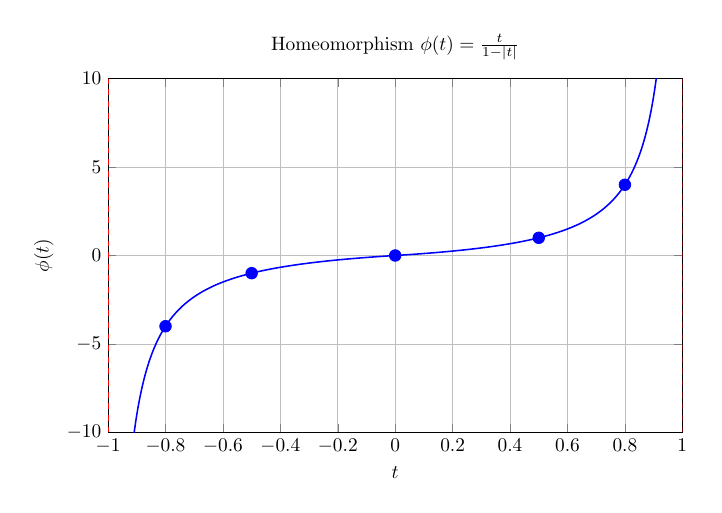
\begin{tikzpicture}[scale=0.7]
        \begin{axis}[
            width=12cm,
            height=8cm,
            xlabel={$t$},
            ylabel={$\phi(t)$},
            xmin=-1, xmax=1,
            ymin=-10, ymax=10,
            grid=major,
            title={Homeomorphism $\phi(t) = \frac{t}{1-|t|}$}
        ]
        
        % Plot the function
        \addplot[blue, thick, samples=1000, domain=-0.99:0.99] {x/(1-abs(x))};
        
        % Mark the asymptotes
        \addplot[dashed, red] coordinates {(-1,-10) (-1,10)};
        \addplot[dashed, red] coordinates {(1,-10) (1,10)};
        
        % Mark some key points
        \addplot[only marks, mark=*, mark size=3pt, blue] coordinates {
            (-0.5,-1) (0,0) (0.5,1) (-0.8,-4) (0.8,4)
        };
        
        \end{axis}
    \end{tikzpicture}
    \caption{The function $\phi(t) = \frac{t}{1-|t|}$ maps the bounded interval $(-1,1)$ bijectively to the unbounded real line $\mathbb{R}$, showing that boundedness is not a topological property.}
    \end{figure}
\bigskip\noindent\textbf{Solution:}
The map $\phi:(-1,1)\to\mathbb{R}$, $\phi(t)=\dfrac{t}{1-|t|}$ is a bijection with continuous inverse $\phi^{-1}(x)=\dfrac{x}{1+|x|}$. Hence a homeomorphism.
\qed

\begin{problembox}[4.35: Space-Filling Curve]
\begin{problemstatement}
Section 9.7 contains an example of a function $f$, continuous on $[0, 1]$, with $f([0, 1]) = [0, 1] \times [0, 1]$. Prove that no such $f$ can be one-to-one on $[0, 1]$.
\end{problemstatement}
\end{problembox}

\noindent\textbf{Strategy:} Use proof by contradiction. Assume $f$ is continuous and injective with image $[0,1]^2$. Remove a point from the interior of the square and show that the remaining set is connected, but removing the corresponding point from $[0,1]$ disconnects it, leading to a contradiction.

\bigskip\noindent\textbf{Solution:}
Suppose $f$ is continuous and injective with image $[0,1]^2$. Remove a point $p\in(0,1)^2$. Then $[0,1]^2\setminus\{p\}$ is connected. But $[0,1]\setminus f^{-1}(p)$ is a disjoint union of two nonempty open intervals (removing any point from $[0,1]$ disconnects it). The continuous bijection $f$ would map this disconnected set onto the connected set $[0,1]^2\setminus\{p\}$, a contradiction. Hence $f$ cannot be one-to-one.\qed

\section{Connectedness}

\begin{definitionssection}{Definitions and Theorems}
\end{definitionssection}

\begin{definition}[Path-Connected Space]
A metric space $S$ is path-connected if for any two points $x,y \in S$ there exists a continuous function $f: [0,1] \to S$ with $f(0) = x$ and $f(1) = y$.
\end{definition}

\noindent\begin{importance}
\textbf{Importance:}Path-connectedness is a stronger form of connectedness that ensures any two points can be joined by a continuous path. It's more intuitive than general connectedness and is often easier to verify in practice. Path-connected spaces are important in many geometric and topological applications.
\end{importance}\begin{theorem}[Connectedness Characterization]
A metric space $S$ is connected if and only if the only subsets of $S$ that are both open and closed are $\emptyset$ and $S$.
\end{theorem}

\noindent\begin{importance}
\textbf{Importance:}This theorem provides a practical way to test for connectedness by checking for "clopen" (closed and open) subsets. It's often easier to work with this characterization than the original definition, especially when proving that spaces are disconnected.
\end{importance}\begin{theorem}[Connected Subsets of $\mathbb{R}$]
The only connected subsets of $\mathbb{R}$ are intervals (including single points and the empty set).
\end{theorem}

\noindent\begin{importance}
\textbf{Importance:}This theorem provides a complete classification of connected subsets of the real line. It's fundamental for understanding the structure of the real numbers and is essential for the intermediate value theorem and many other results in analysis.
\end{importance}\begin{theorem}[Closure of Connected Set]
The closure of a connected set is connected.
\end{theorem}

\noindent\begin{importance}
\textbf{Importance:}This theorem shows that connectedness is preserved when taking closures, which is important for many applications where we need to work with closed sets or complete spaces. It's particularly useful in analysis where we often need to consider closures of sets.
\end{importance}
\begin{problembox}[4.36: Disconnected Metric Spaces]
\begin{problemstatement}
Prove that a metric space $S$ is disconnected if, and only if, there is a nonempty subset $A$ of $S$, $A \neq S$, which is both open and closed in $S$.
\end{problemstatement}
\end{problembox}

\noindent\textbf{Strategy:} Use the definition of disconnectedness and the fact that a set is both open and closed if and only if its complement is also both open and closed. If $S$ is disconnected, write it as a union of two disjoint nonempty open sets, then one of them serves as the required subset.

\bigskip\noindent\textbf{Solution:}
If $S$ is disconnected, write $S=U\cup V$ with disjoint nonempty open sets. Then $U$ is open and closed (its complement $V$ is open). Conversely, if $A$ is nonempty, proper, open and closed, then $S=A\cup(S\setminus A)$ is a separation, so $S$ is disconnected.\qed

\begin{problembox}[4.37: Connected Metric Spaces]
\begin{problemstatement}
Prove that a metric space $S$ is connected if, and only if, the only subsets of $S$ which are both open and closed in $S$ are the empty set and $S$ itself.
\end{problemstatement}
\end{problembox}

\noindent\textbf{Strategy:} This is the contrapositive of Exercise 4.36. A space is connected if and only if it is not disconnected, which means there are no nontrivial clopen subsets.

\bigskip\noindent\textbf{Solution:}
This is the contrapositive of 4.36: connectedness is equivalent to having no nontrivial clopen subsets.\qed

\begin{problembox}[4.38: Connected Subsets of Reals]
\begin{problemstatement}
Prove that the only connected subsets of $\mathbb{R}$ are:
\begin{enumerate}[label=(\alph*)]
\item the empty set,
\item sets consisting of a single point, and
\item intervals (open, closed, half-open, or infinite).
\end{enumerate}
\end{problemstatement}
\end{problembox}

\noindent\textbf{Strategy:} We need to prove two directions: (1) If a subset of $\mathbb{R}$ is connected, then it must be empty, a single point, or an interval. (2) If a subset is empty, a single point, or an interval, then it is connected. For the first direction, we'll use proof by contradiction - if a connected set contains two points but misses a point between them, we can create a separation. For the second direction, we'll show that intervals cannot be separated into two disjoint open sets.

\bigskip\noindent\textbf{Solution:}

\textbf{Forward direction:} Let $E \subset \mathbb{R}$ be connected. If $E$ is empty or contains only one point, we're done. Suppose $E$ contains at least two points $a < b$. We need to show that $E$ contains all points between $a$ and $b$.

Suppose for contradiction that there exists $c \in (a,b)$ such that $c \notin E$. Then we can write $E$ as the union of two disjoint nonempty sets:
\[E = (E \cap (-\infty, c)) \cup (E \cap (c, \infty))\]

Since $a \in E \cap (-\infty, c)$ and $b \in E \cap (c, \infty)$, both sets are nonempty. Also, $(-\infty, c)$ and $(c, \infty)$ are open sets in $\mathbb{R}$, so their intersections with $E$ are relatively open in $E$. This gives us a separation of $E$, contradicting the assumption that $E$ is connected.

Therefore, if $E$ contains two points $a < b$, it must contain all points in $[a,b]$. This means $E$ is an interval (which includes all types: open, closed, half-open, and infinite intervals).

\textbf{Reverse direction:} Now we show that intervals are connected. Let $I$ be an interval in $\mathbb{R}$. Suppose for contradiction that $I$ is disconnected, so $I = U \cup V$ where $U$ and $V$ are disjoint nonempty relatively open sets.

Let $a \in U$ and $b \in V$. Without loss of generality, assume $a < b$. Since $I$ is an interval, $[a,b] \subset I$. Let $c = \sup\{x \in U : x < b\}$. Since $U$ is relatively open, $c \in U$ (otherwise there would be a sequence in $U$ converging to $c$, but $c \notin U$, contradicting that $U$ is closed in the subspace topology).

Now consider any point $d$ with $c < d < b$. Since $d > c = \sup\{x \in U : x < b\}$, we must have $d \in V$. But this means that in any neighborhood of $c$, there are points from both $U$ and $V$, which contradicts the fact that $U$ and $V$ are disjoint open sets.

Therefore, intervals cannot be disconnected, so they are connected.

We have shown that the only connected subsets of $\mathbb{R}$ are the empty set, single points, and intervals.\qed

\begin{problembox}[4.39: Connectedness of Intermediate Sets]
\begin{problemstatement}
Let $X$ be a connected subset of a metric space $S$. Let $Y$ be a subset of $S$ such that $X \subseteq Y \subseteq \overline{X}$, where $\overline{X}$ is the closure of $X$. Prove that $Y$ is also connected. In particular, this shows that $\overline{X}$ is connected.
\end{problemstatement}
\end{problembox}

\noindent\textbf{Strategy:} Use proof by contradiction. If $Y$ were disconnected, it could be written as a union of two disjoint nonempty relatively open sets. The intersection of these sets with $X$ would form a separation of $X$, contradicting the connectedness of $X$.

\bigskip\noindent\textbf{Solution:}
If $Y$ were disconnected, write $Y=U\cup V$ with disjoint nonempty sets open in the subspace topology. Then $U\cap X$ and $V\cap X$ would form a separation of $X$ (they are relatively open and disjoint, and cover $X$), contradicting connectedness of $X$. Thus $Y$ is connected.\qed

\begin{problembox}[4.40: Closed Components]
\begin{problemstatement}
If $x$ is a point in a metric space $S$, let $U(x)$ be the component of $S$ containing $x$. Prove that $U(x)$ is closed in $S$.
\end{problemstatement}
\end{problembox}

\noindent\textbf{Strategy:} Use the fact that the closure of a connected set is connected. If a sequence in $U(x)$ converges to a point $y$, then $y$ must belong to the closure of $U(x)$, which is connected and contains $x$, hence $y \in U(x)$.

\bigskip\noindent\textbf{Solution:}
Let $(x_n)\subset U(x)$ with $x_n\to y\in S$. For each $n$, $x_n$ lies in the (maximal) connected set $U(x)$. The closure of a connected set is connected, and $y\in\overline{U(x)}$. The component containing $x$ is closed under taking limits of sequences within it; more directly, the union of all connected subsets containing $x$ is closed, hence $y\in U(x)$. Therefore $U(x)$ is closed.\qed

\begin{problembox}[4.41: Components of Open Sets in $\mathbb{R}$]
\begin{problemstatement}
Let $S$ be an open subset of $\mathbb{R}$. By Theorem 3.11, $S$ is the union of a countable disjoint collection of open intervals in $\mathbb{R}$. Prove that each of these open intervals is a component of the metric subspace $S$. Explain why this does not contradict Exercise 4.40.
\end{problemstatement}
\end{problembox}

\noindent\textbf{Strategy:} Use the fact that open intervals are connected and maximal within $S$ (any larger subset would cross a gap and disconnect). For the apparent contradiction, note that components are closed in the subspace topology on $S$, not necessarily in the ambient space $\mathbb{R}$.

\bigskip\noindent\textbf{Solution:}
Each open interval is connected and maximal (any strictly larger subset within $S$ would cross a gap and disconnect), hence is a component. This does not contradict 4.40 because components are closed \emph{in the subspace topology on $S$}, and an open interval is closed in $S$ though not closed in $\mathbb{R}$.\qed

\begin{problembox}[4.42: $\varepsilon$-Chain Connectedness]
\begin{problemstatement}
Given a compact set $S$ in $\mathbb{R}^m$ with the following property: For every pair of points $a$ and $b$ in $S$ and for every $\varepsilon > 0$ there exists a finite set of points $(x_0, x_1, \ldots, x_n)$ in $S$ with $x_0 = a$ and $x_n = b$ such that
\[\|x_k - x_{k-1}\| < \varepsilon \quad \text{for } k = 1, 2, \ldots, n.\]
Prove or disprove: $S$ is connected.
\end{problemstatement}
\end{problembox}

\noindent\textbf{Strategy:} Use proof by contradiction. If $S$ were disconnected, it could be written as a union of two disjoint nonempty closed sets. By compactness, the distance between these sets is positive, and taking $\varepsilon$ smaller than this distance would prevent any $\varepsilon$-chain from connecting points in different components.

\bigskip\noindent\textbf{Solution:}
True. Suppose $S=A\cup B$ with disjoint nonempty closed sets. Let $\delta=\mathrm{dist}(A,B)>0$ (positive by compactness). Taking $\varepsilon<\delta$, no $\varepsilon$-chain can go from $A$ to $B$, contradicting the hypothesis. Hence $S$ is connected.\qed

\begin{problembox}[4.43: Boundary Characterization of Connectedness]
\begin{problemstatement}
Prove that a metric space $S$ is connected if, and only if, every nonempty proper subset of $S$ has a nonempty boundary.
\end{problemstatement}
\end{problembox}

\noindent\textbf{Strategy:} Use the fact that the boundary of a set $A$ is $\partial A = \overline{A} \cap \overline{S \setminus A}$. If $S$ is connected, then for any proper subset $A$, both $\overline{A}$ and $\overline{S \setminus A}$ must meet, giving a nonempty boundary. For the converse, if some set has empty boundary, it is both open and closed, creating a separation.

\bigskip\noindent\textbf{Solution:}
If $S$ is connected and $\emptyset\ne A\subsetneq S$, then both $\overline{A}$ and $\overline{S\setminus A}$ meet, so $\partial A=\overline{A}\cap\overline{S\setminus A}\ne\emptyset$. Conversely, if some $A$ has empty boundary, then $A$ is both open and closed, giving a separation; thus $S$ would be disconnected.\qed

\begin{problembox}[4.44: Convex Implies Connected]
\begin{problemstatement}
Prove that every convex subset of $\mathbb{R}^n$ is connected.
\end{problemstatement}
\end{problembox}

\noindent\textbf{Strategy:} Use the definition of convexity: for any two points $x, y$ in a convex set $C$, the line segment joining them is contained in $C$. Since line segments are connected and any two points can be joined by a connected subset, the set is connected.

\bigskip\noindent\textbf{Solution:}
If $C$ is convex and $x,y\in C$, then the line segment $\{tx+(1-t)y: t\in[0,1]\}\subset C$ is connected. Since any two points can be joined by a connected subset, $C$ is connected.\qed

\begin{problembox}[4.45: Image of Disconnected Sets]
\begin{problemstatement}
Given a function $f : \mathbb{R}^n \to \mathbb{R}^m$ which is one-to-one and continuous on $\mathbb{R}^n$. If $A$ is open and disconnected in $\mathbb{R}^n$, prove that $f(A)$ is open and disconnected in $\mathbb{R}^m$.
\end{problemstatement}
\end{problembox}

\noindent\textbf{Strategy:} Use the invariance of domain theorem which states that an injective continuous map from $\mathbb{R}^n$ to itself is open. If $A = U \cup V$ is a separation, then $f(U)$ and $f(V)$ are disjoint open sets whose union is $f(A)$, making $f(A)$ disconnected.

\bigskip\noindent\textbf{Solution:}
Assume $n=m$. By invariance of domain, an injective continuous map $f:\mathbb{R}^n\to\mathbb{R}^n$ is open, hence $f(A)$ is open. If $A=U\cup V$ is a separation, then $f(U)$ and $f(V)$ are disjoint open sets whose union is $f(A)$; thus $f(A)$ is disconnected. (If $m\ne n$, openness need not hold.)\qed

\begin{problembox}[4.46: Topologist's Sine Curve]
\begin{problemstatement}
Let $A = \{(x, y) : 0 < x \leq 1, y = \sin(1/x)\}$, $B = \{(x, y) : y = 0, -1 \leq x \leq 0\}$, and let $S = A \cup B$. Prove that $S$ is connected but not arcwise connected.
\end{problemstatement}
\end{problembox}

\noindent\textbf{Strategy:} Show connectedness by using the fact that the closure of $A$ includes the vertical segment $\{0\} \times [-1,1]$, making $S$ connected. For path-disconnectedness, show that any continuous path from $(0,0)$ to a point in $A$ would have to intersect infinitely many oscillations of the sine curve, which is impossible for a compact path.

% Topologist's sine curve S = A ∪ B
% A = {(x, sin(1/x)) : 0 < x ≤ 1},  B = {(x,0) : -1 ≤ x ≤ 0}
% Dashed vertical segment at x=0 shows the closure limit set {0}×[-1,1] (for intuition).

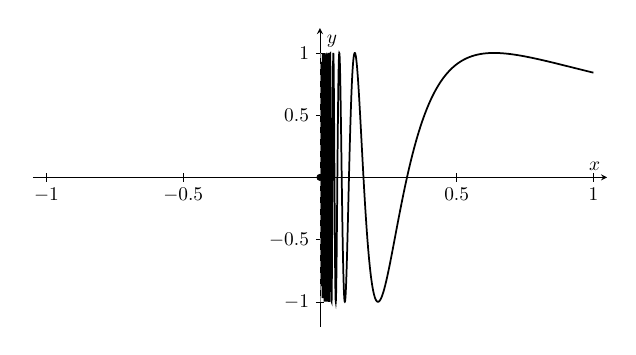
\begin{tikzpicture}[scale=0.7]
    \begin{axis}[
      axis lines=middle,
      xlabel={$x$}, ylabel={$y$},
      xmin=-1.05, xmax=1.05,
      ymin=-1.2,  ymax=1.2,
      width=12cm, height=7cm,
      xtick={-1,-0.5,0,0.5,1},
      ytick={-1,-0.5,0,0.5,1},
      tick style={black},
      domain=0.005:1
    ]
    
    % The oscillatory set A: y = sin(1/x) for 0 < x ≤ 1
    \addplot[
      smooth,
      samples=2200,
      line width=0.9pt
    ]
    {x <= 0 ? nan : sin(deg(1/x))};
    
    % The horizontal segment B on the left: y = 0, -1 ≤ x ≤ 0
    \addplot[
      line width=0.9pt
    ]
    table[row sep=\\]{
    -1 0 \\
     0 0 \\
    };
    
    % Show the closure's limit set at x=0 (not part of S): {0}×[-1,1]
    \addplot[
      dashed,
      gray
    ]
    table[row sep=\\]{
    0 -1 \\
    0  1 \\
    };
    
    % Emphasize the shared point (0,0) (belongs to B but not to A)
    \addplot[
      only marks, mark=*, mark size=1.6pt
    ]
    coordinates {(0,0)};
    
    \end{axis}
    \end{tikzpicture}
    

\bigskip\noindent\textbf{Solution:}
The closure of $A$ adds the vertical segment $\{0\}\times[-1,1]$. The set $S$ equals $A$ together with a horizontal segment adjoining at the origin; $S$ is connected as the continuous image of $(0,1]\cup[-1,0]$ under a map gluing at the origin, or via boundary characterization. However, there is no continuous injective path in $S$ from $(0,0)$ to any point of $A$ (an arc would intersect infinitely many oscillations, forcing a contradiction with compactness of arcs). Thus $S$ is not arcwise connected.\qed

\begin{problembox}[4.47: Nested Connected Compact Sets]
\begin{problemstatement}
Let $F = (F_1, F_2, \ldots)$ be a countable collection of connected compact sets in $\mathbb{R}^s$ such that $F_{k+1} \subseteq F_k$ for each $k \geq 1$. Prove that the intersection $\bigcap_{k=1}^{\infty} F_k$ is connected and closed.
\end{problemstatement}
\end{problembox}

\noindent\textbf{Strategy:} Use the fact that the intersection of compact sets is compact (hence closed). For connectedness, use proof by contradiction: if the intersection were disconnected, there would exist disjoint open sets separating it, but each $F_k$ is connected and contains the intersection, so it must lie entirely in one of the open sets, leading to a contradiction.

\bigskip\noindent\textbf{Solution:}
The intersection of compact sets is compact (hence closed). If the intersection were disconnected, write it as $K\cup L$ with disjoint nonempty closed sets. By compactness, there exist disjoint open sets $U,V$ with $K\subset U$, $L\subset V$. For each $k$, $F_k$ is connected and contains $K\cup L$, so $F_k\subset U\cup V$ forces $F_k\subset U$ or $F_k\subset V$, impossible since both $K$ and $L$ are contained in the intersection. Hence the intersection is connected.\qed

\begin{problembox}[4.48: Complement of Components]
\begin{problemstatement}
Let $S$ be an open connected set in $\mathbb{R}^n$. Let $T$ be a component of $\mathbb{R}^n \setminus S$. Prove that $\mathbb{R}^n \setminus T$ is connected.
\end{problemstatement}
\end{problembox}

\noindent\textbf{Strategy:} Use proof by contradiction. If $\mathbb{R}^n \setminus T$ were disconnected, it could be written as a union of two disjoint nonempty open sets. Since $S$ is connected and contained in $\mathbb{R}^n \setminus T$, it must lie entirely in one of these sets, but this would create a separation of the boundary of $T$, which is impossible.

\bigskip\noindent\textbf{Solution:}
Assume $\mathbb{R}^n\setminus T=U\cup V$ is disconnected. Since $S\subset\mathbb{R}^n\setminus T$, $S$ must lie entirely in $U$ or $V$; say $S\subset U$. Then $V\subset \mathbb{R}^n\setminus S$ is open and nonempty, and each component of $\mathbb{R}^n\setminus S$ must be contained in $V$ or in the complement of $V$, contradicting that $T$ meets both sides of the separation. A boundary-based argument shows any separation would separate the connected boundary $\partial T\subset S$, impossible. Thus $\mathbb{R}^n\setminus T$ is connected.\qed

\begin{problembox}[4.49: Unbounded Connected Spaces]
\begin{problemstatement}
Let $(S, d)$ be a connected metric space which is not bounded. Prove that for every $a$ in $S$ and every $r > 0$, the set $\{x : d(x, a) = r\}$ is nonempty.
\end{problemstatement}
\end{problembox}

\noindent\textbf{Strategy:} Use the fact that the distance function $x \mapsto d(x,a)$ is continuous from $S$ to $[0,\infty)$. Since $S$ is connected and unbounded, the image of this function must be a connected unbounded subset of $[0,\infty)$ containing $0$, which must be the entire interval $[0,\infty)$.

\bigskip\noindent\textbf{Solution:}
The map $x\mapsto d(x,a)$ is continuous $S\to[0,\infty)$. Since $S$ is connected and unbounded, its image is a connected unbounded subset of $[0,\infty)$ containing $0$, hence equals $[0,\infty)$. Therefore each $r>0$ is attained.\qed

\section{Uniform Continuity}

\begin{definitionssection}{Definitions and Theorems}
\end{definitionssection}

\begin{definition}[Uniform Continuity]
A function $f: S \to T$ between metric spaces is uniformly continuous if for every $\varepsilon > 0$ there exists $\delta > 0$ such that $d_S(x,y) < \delta$ implies $d_T(f(x), f(y)) < \varepsilon$ for all $x,y \in S$.
\end{definition}

\noindent\begin{importance}
\textbf{Importance:}Uniform continuity is a stronger form of continuity that ensures the same $\delta$ works for all points in the domain. This is crucial for many applications where we need to control the behavior of functions uniformly across their entire domain, such as in integration theory and approximation theory.
\end{importance}\begin{definition}[Lipschitz Functions]
A function $f: S \to T$ between metric spaces is called Lipschitz continuous (or simply Lipschitz) if there exists a constant $L > 0$ such that for all $x, y \in S$,
\[d_T(f(x), f(y)) \leq L \cdot d_S(x, y).\]
The smallest such constant $L$ is called the Lipschitz constant of $f$. If $L = 1$, we say $f$ is 1-Lipschitz or nonexpansive.
\end{definition}

\noindent\begin{importance}
\textbf{Importance:}Lipschitz functions provide a quantitative measure of how much a function can stretch distances. They are automatically uniformly continuous and play a crucial role in analysis, optimization, and differential equations. The 1-Lipschitz property means the function never increases distances between points.
\end{importance}\begin{theorem}[Uniform Continuity on Compact Sets]
A continuous function on a compact metric space is uniformly continuous.
\end{theorem}

\noindent\begin{importance}
\textbf{Importance:}This is one of the most important theorems in analysis, showing that on compact domains, the stronger property of uniform continuity comes "for free" from ordinary continuity. This is essential for many applications in calculus, integration, and approximation theory.
\end{importance}\begin{theorem}[Distance Function Properties]
Let $A$ be a nonempty subset of a metric space $(S,d)$. The distance function $f_A(x) = \inf\{d(x,y) : y \in A\}$ is uniformly continuous and satisfies $\overline{A} = \{x : f_A(x) = 0\}$.
\end{theorem}

\noindent\begin{importance}
\textbf{Importance:}This theorem shows that distance functions are well-behaved and provides a useful tool for characterizing closures of sets. The uniform continuity of distance functions makes them valuable in many applications, particularly in optimization and approximation theory.
\end{importance}\begin{theorem}[Urysohn's Lemma]
Let $A$ and $B$ be disjoint closed subsets of a metric space $(S,d)$. Then there exist disjoint open sets $U$ and $V$ such that $A \subseteq U$ and $B \subseteq V$.
\end{theorem}

\noindent\begin{importance}
\textbf{Importance:}This is a fundamental result in topology that shows metric spaces have good separation properties. It's essential for constructing continuous functions with specific properties and is the foundation for many results in functional analysis and topology.
\end{importance}
\begin{problembox}[4.50: Uniform Implies Continuous]
\begin{problemstatement}
Prove that a function which is uniformly continuous on $S$ is also continuous on $S$.
\end{problemstatement}
\end{problembox}

\noindent\textbf{Strategy:} Use the definitions directly. Uniform continuity provides a $\delta$ that works for all points simultaneously, which immediately implies continuity at each individual point.

\bigskip\noindent\textbf{Solution:}
Immediate from the definitions: given $\varepsilon>0$, pick $\delta$ working for all points; then continuity at each point follows.\qed

\begin{problembox}[4.51: Non-Uniform Continuity Example]
\begin{problemstatement}
If $f(x) = x^2$ for $x$ in $\mathbb{R}$, prove that $f$ is not uniformly continuous on $\mathbb{R}$.
\end{problemstatement}
\end{problembox}

\noindent\textbf{Strategy:} Use proof by contradiction. Assume uniform continuity and find a contradiction by choosing specific points where the difference in function values exceeds any given $\varepsilon$ while the difference in arguments is less than any given $\delta$.

\bigskip\noindent\textbf{Solution:}
For $\varepsilon=1$, any $\delta>0$ fails by choosing $x=1/\delta$ and $y=x+\tfrac{\delta}{2}$: then $|x-y|<\delta$ but $|x^2-y^2|=|x-y||x+y|>\tfrac{\delta}{2}\cdot\tfrac{2}{\delta}=1$.\qed

\begin{problembox}[4.52: Boundedness of Uniformly Continuous Functions]
\begin{problemstatement}
Assume that $f$ is uniformly continuous on a bounded set $S$ in $\mathbb{R}^n$. Prove that $f$ must be bounded on $S$.
\end{problemstatement}
\end{problembox}

\noindent\textbf{Strategy:} Use the uniform continuity condition to cover $S$ with finitely many balls of radius $\delta$. Since $S$ is bounded, it can be covered by finitely many such balls, and the image of each ball is bounded by continuity at its center.

\bigskip\noindent\textbf{Solution:}
Cover $S$ by finitely many balls of radius $\delta$ from the uniform continuity condition for $\varepsilon=1$. The image of each ball is bounded (by continuity at its center). The finite union is bounded.\qed

\begin{problembox}[4.53: Composition of Uniformly Continuous Functions]
\begin{problemstatement}
Let $f$ be a function defined on a set $S$ in $\mathbb{R}^n$ and assume that $f(S) \subseteq \mathbb{R}^m$. Let $g$ be defined on $f(S)$ with value in $\mathbb{R}^k$, and let $h$ denote the composite function defined by $h(x) = g[f(x)]$ if $x \in S$. If $f$ is uniformly continuous on $S$ and if $g$ is uniformly continuous on $f(S)$, show that $h$ is uniformly continuous on $S$.
\end{problemstatement}
\end{problembox}

\noindent\textbf{Strategy:} Use the uniform continuity conditions for both $f$ and $g$. Given $\varepsilon > 0$, first find $\eta > 0$ for $g$, then find $\delta > 0$ for $f$ such that when $x$ and $x'$ are close, their images under $f$ are close enough for $g$ to preserve the $\varepsilon$ condition.

\bigskip\noindent\textbf{Solution:}
Given $\varepsilon>0$, pick $\eta>0$ for $g$ on $f(S)$; pick $\delta>0$ for $f$ such that $\|x-x'\|<\delta\Rightarrow \|f(x)-f(x')\|<\eta$. Then $\|x-x'\|<\delta\Rightarrow \|h(x)-h(x')\|=\|g(f(x))-g(f(x'))\|<\varepsilon$.\qed

\begin{problembox}[4.54: Preservation of Cauchy Sequences]
\begin{problemstatement}
Assume $f : S \to T$ is uniformly continuous on $S$, where $S$ and $T$ are metric spaces. If $(x_n)$ is any Cauchy sequence in $S$, prove that $(f(x_n))$ is a Cauchy sequence in $T$. (Compare with Exercise 4.33.)
\end{problemstatement}
\end{problembox}

\noindent\textbf{Strategy:} Use the uniform continuity condition to find $\delta > 0$ for a given $\varepsilon > 0$. Since $(x_n)$ is Cauchy, there exists $N$ such that for $n, m \geq N$, the distance between $x_n$ and $x_m$ is less than $\delta$, which implies the distance between $f(x_n)$ and $f(x_m)$ is less than $\varepsilon$.

\bigskip\noindent\textbf{Solution:}
Given $\varepsilon>0$, by uniform continuity choose $\delta>0$ such that $d_S(x,y)<\delta\Rightarrow d_T(f(x),f(y))<\varepsilon$. Since $(x_n)$ is Cauchy, there exists $N$ with $d_S(x_n,x_m)<\delta$ for $n,m\ge N$. Hence $d_T(f(x_n),f(x_m))<\varepsilon$ for $n,m\ge N$.\qed

\begin{problembox}[4.55: Uniform Continuous Extension]
\begin{problemstatement}
Let $f : S \to T$ be a function from a metric space $S$ to another metric space $T$. Assume $f$ is uniformly continuous on a subset $A$ of $S$ and that $T$ is complete. Prove that there is a unique extension of $f$ to $\overline{A}$ which is uniformly continuous on $\overline{A}$.
\end{problemstatement}
\end{problembox}

\noindent\textbf{Strategy:} Use the fact that any point in $\overline{A}$ is the limit of a sequence in $A$. By Exercise 4.54, the image sequence is Cauchy and converges in the complete space $T$. Define the extension as the limit of these sequences and show it's well-defined and uniformly continuous.

\bigskip\noindent\textbf{Solution:}
For $x\in\overline{A}$ choose any sequence $(a_n)\subset A$ with $a_n\to x$. Then $(f(a_n))$ is Cauchy by 4.54, hence convergent in complete $T$. Define $\tilde f(x)=\lim f(a_n)$. This is well-defined (limits coincide for different sequences by interlacing and uniform continuity). Then $\tilde f$ extends $f$ and is uniformly continuous: given $\varepsilon>0$, pick $\delta$ for $f$ on $A$; approximate points in $\overline{A}$ by nearby points in $A$ and pass to limits.\qed

\begin{problembox}[4.56: Distance Function]
\begin{problemstatement}
In a metric space $(S, d)$, let $A$ be a nonempty subset of $S$. Define a function $f_A : S \to \mathbb{R}$ by the equation
\[f_A(x) = \inf \{d(x, y) : y \in A\}\]
for each $x$ in $S$. The number $f_A(x)$ is called the distance from $x$ to $A$.
\begin{enumerate}[label=(\alph*)]
\item Prove that $f_A$ is uniformly continuous on $S$.
\item Prove that $\overline{A} = \{x : x \in S \text{ and } f_A(x) = 0\}$.
\end{enumerate}
\end{problemstatement}
\end{problembox}

\noindent\textbf{Strategy:} For (a), use the reverse triangle inequality to show that $|f_A(x) - f_A(z)| \leq d(x,z)$, making $f_A$ 1-Lipschitz and hence uniformly continuous. For (b), use the definition of closure: $x \in \overline{A}$ if and only if there exists a sequence in $A$ converging to $x$, which is equivalent to $f_A(x) = 0$.

\bigskip\noindent\textbf{Solution:}
(a) For all $x,z$ and $y\in A$, $|d(x,y)-d(z,y)|\le d(x,z)$. Taking infimum over $y$ gives $|f_A(x)-f_A(z)|\le d(x,z)$, so $f_A$ is $1$-Lipschitz.

(b) If $x\in\overline{A}$, there exist $y_n\in A$ with $d(x,y_n)\to 0$, so $f_A(x)=0$. Conversely, if $f_A(x)=0$, pick $y_n\in A$ with $d(x,y_n)<1/n$; then $y_n\to x$, hence $x\in\overline{A}$.\qed

\begin{problembox}[4.57: Separation by Open Sets]
\begin{problemstatement}
In a metric space $(S, d)$, let $A$ and $B$ be disjoint closed subsets of $S$. Prove that there exist disjoint open subsets $U$ and $V$ of $S$ such that $A \subseteq U$ and $B \subseteq V$. \\
\textit{Hint.} Let $g(x) = f_A(x) - f_B(x)$, in the notation of Exercise 4.56, and consider $g^{-1}(-\infty, 0)$ and $g^{-1}(0, +\infty)$.
\end{problemstatement}
\end{problembox}

\noindent\textbf{Strategy:} Use the hint to define $g(x) = f_A(x) - f_B(x)$, which is continuous as a difference of continuous functions. The sets $U = \{g < 0\}$ and $V = \{g > 0\}$ are open and disjoint, with $A \subseteq U$ and $B \subseteq V$ by the properties of the distance functions.

\bigskip\noindent\textbf{Solution:}
Define $g(x)=f_A(x)-f_B(x)$, which is continuous as a difference of Lipschitz functions. Then $U=\{g<0\}$ and $V=\{g>0\}$ are disjoint open sets containing $A$ and $B$ respectively.\qed

\section{Discontinuities}

\begin{definitionssection}{Definitions and Theorems}
\end{definitionssection}

\begin{definition}[Types of Discontinuities]
Let $f$ be defined on an interval containing $c$ except possibly at $c$ itself.
\begin{enumerate}
\item $f$ has a removable discontinuity at $c$ if $\lim_{x \to c} f(x)$ exists but is not equal to $f(c)$
\item $f$ has a jump discontinuity at $c$ if both one-sided limits exist but are not equal
\item $f$ has an essential discontinuity at $c$ if at least one one-sided limit does not exist
\end{enumerate}
\end{definition}

\noindent\begin{importance}
\textbf{Importance:}This classification provides a systematic way to understand and categorize the different ways functions can fail to be continuous. It's essential for understanding the behavior of functions near problematic points and for developing techniques to handle discontinuities in analysis and applications.
\end{importance}
\begin{problembox}[4.58: Classification of Discontinuities]
\begin{problemstatement}
Locate and classify the discontinuities of the functions $f$ defined on $\mathbb{R}^1$ by the following equations:
\begin{enumerate}[label=(\alph*)]
\item $f(x) = (\sin x)/x$ if $x \neq 0$, $f(0) = 0$.
\item $f(x) = e^{1/x}$ if $x \neq 0$, $f(0) = 0$.
\item $f(x) = e^{1/x} + \sin(1/x)$ if $x \neq 0$, $f(0) = 0$.
\item $f(x) = 1/(1 - e^{1/x})$ if $x \neq 0$, $f(0) = 0$.
\end{enumerate}
\end{problemstatement}
\end{problembox}

\noindent\textbf{Strategy:} For each function, analyze the behavior as $x \to 0$ from both positive and negative directions. Check if the limit exists and equals the function value (removable), if one-sided limits exist but differ (jump), or if at least one one-sided limit doesn't exist (essential).
% Plot showing different types of discontinuities
\begin{figure}[h!]
    \centering
    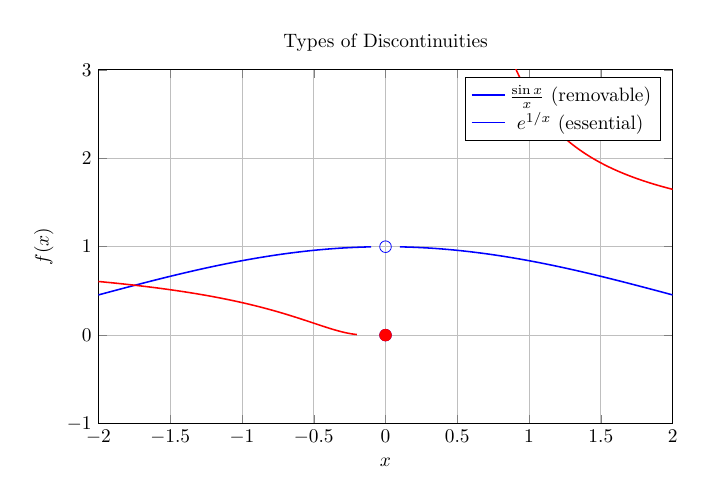
\begin{tikzpicture}[scale=0.7]
        \begin{axis}[
            width=12cm,
            height=8cm,
            xlabel={$x$},
            ylabel={$f(x)$},
            xmin=-2, xmax=2,
            ymin=-1, ymax=3,
            grid=major,
            title={Types of Discontinuities}
        ]
        
        % (a) Removable discontinuity: sin(x)/x
        \addplot[blue, thick, samples=100, domain=-2:-0.1] {sin(deg(x))/x};
        \addplot[blue, thick, samples=100, domain=0.1:2] {sin(deg(x))/x};
        \addplot[only marks, mark=*, mark size=3pt, blue] coordinates {(0,0)};
        \addplot[only marks, mark=o, mark size=3pt, blue] coordinates {(0,1)};
        \addlegendentry{$\frac{\sin x}{x}$ (removable)}
        
        % (b) Essential discontinuity: e^(1/x)
        \addplot[red, thick, samples=200, domain=0.2:2] {exp(1/x)};
        \addplot[red, thick, samples=200, domain=-2:-0.2] {exp(1/x)};
            \addplot[only marks, mark=*, mark size=3pt, red] coordinates {(0,0)};
        \addlegendentry{$e^{1/x}$ (essential)}
        \end{axis}
    \end{tikzpicture}
    \caption{Examples of removable discontinuity ($sin(x)/x$ at $x=0$) and essential discontinuity ($e^(1/x)$ at $x=0$). The removable discontinuity can be fixed by redefining the function value.}
    \end{figure}

\bigskip\noindent\textbf{Solution:}
(a) Removable at $0$: $\lim_{x\to0}(\sin x)/x=1\ne f(0)$; redefining $f(0)=1$ yields continuity.

(b) Essential at $0$: along $x\to 0^+$, $e^{1/x}\to+\infty$; along $x\to0^-$, $e^{1/x}\to 0$. No finite limit; discontinuity of essential type.

(c) Essential at $0$: the term $e^{1/x}$ behaves as in (b) and $\sin(1/x)$ oscillates; no limit exists.

(d) Essential at $0$: as $x\to0^-$, $e^{1/x}\to0$ so $f\to 1$; as $x\to0^+$, $e^{1/x}\to+\infty$ and $f\to 0$ except near points where $e^{1/x}=1$ causing poles; thus infinitely many essential singularities accumulating at $0$; no limit.


\qed

\begin{problembox}[4.59: Discontinuities in $\mathbb{R}^2$]
\begin{problemstatement}
Locate the points in $\mathbb{R}^2$ at which each of the functions in Exercise 4.11 is not continuous.
\end{problemstatement}
\end{problembox}

\noindent\textbf{Strategy:} This problem refers to Exercise 4.11 which doesn't contain specific functions in this text. If concrete functions were provided, analyze continuity by examining limits along different curves approaching the points of interest, particularly checking if the limit depends on the path taken.

\bigskip\noindent\textbf{Solution:}
Not applicable as stated here: Exercise 4.11 in this text does not list specific functions. If concrete functions are provided, analyze continuity by examining limits along curves approaching the points of interest.\qed

\section{Monotonic Functions}

\begin{definitionssection}{Definitions and Theorems}
\end{definitionssection}

\begin{definition}[Monotonic Function]
A function $f: [a,b] \to \mathbb{R}$ is:
\begin{enumerate}
\item Increasing if $x < y$ implies $f(x) \leq f(y)$
\item Strictly increasing if $x < y$ implies $f(x) < f(y)$
\item Decreasing if $x < y$ implies $f(x) \geq f(y)$
\item Strictly decreasing if $x < y$ implies $f(x) > f(y)$
\end{enumerate}
\end{definition}

\noindent\begin{importance}
\textbf{Importance:}Monotonic functions have many desirable properties that make them easier to work with than general functions. They have well-behaved limits, countable discontinuities, and preserve order. These properties make them fundamental in analysis, optimization, and many applications.
\end{importance}\begin{theorem}[Monotonic Function Properties]
Let $f$ be monotonic on $[a,b]$. Then:
\begin{enumerate}
\item $f$ has one-sided limits at every point in $(a,b)$
\item The set of discontinuities of $f$ is countable
\item $f$ has points of continuity in every open subinterval
\end{enumerate}
\end{theorem}

\noindent\begin{importance}
\textbf{Importance:}This theorem provides fundamental properties of monotonic functions that make them much more manageable than general functions. The fact that discontinuities are countable and that continuity points are dense makes monotonic functions essential in many areas of analysis and applications.
\end{importance}
\begin{problembox}[4.60: Local Increasing Implies Increasing]
\begin{problemstatement}
Let $f$ be defined in the open interval $(a, b)$ and assume that for each interior point $x$ of $(a, b)$ there exists a 1-ball $B(x)$ in which $f$ is increasing. Prove that $f$ is an increasing function throughout $(a, b)$.
\end{problemstatement}
\end{problembox}

\noindent\textbf{Strategy:} Use the compactness property of closed intervals. For any two points $u < v$ in $(a,b)$, construct a finite chain connecting them where each segment lies within one of the local increasing balls, then use the increasing property on each segment to show $f(u) \leq f(v)$.

\bigskip\noindent\textbf{Solution:}
Fix $u<v$ in $(a,b)$. Connect $u$ to $v$ by a finite chain $u=x_0<x_1<\cdots<x_k=v$ with $[x_{i-1},x_i]\subset B(t_i)$ for suitable centers $t_i$. On each $[x_{i-1},x_i]$, $f$ is increasing, hence $f(u)\le f(x_1)\le\cdots\le f(v)$. Thus $f$ is increasing on $(a,b)$.\qed

\begin{problembox}[4.61: No Local Extrema Implies Monotonic]
\begin{problemstatement}
Let $f$ be continuous on a compact interval $[a, b]$ and assume that $f$ does not have a local maximum or a local minimum at any interior point. Prove that $f$ must be monotonic on $[a, b]$.
\end{problemstatement}
\end{problembox}

\noindent\textbf{Strategy:} Use the extreme value theorem to show that $f$ attains its maximum and minimum at the endpoints since there are no interior local extrema. This forces the function to be either nondecreasing or nonincreasing, and the intermediate value property excludes oscillation.

\bigskip\noindent\textbf{Solution:}
By the extreme value theorem, $f$ attains its maximum and minimum at endpoints since there are no interior local extrema. Therefore either $f(a)\le f(b)$ and $f$ is nondecreasing, or $f(a)\ge f(b)$ and $f$ is nonincreasing. A standard argument via the intermediate value property excludes oscillation without local extrema.\qed

\begin{problembox}[4.62: One-to-One Continuous Implies Strictly Monotonic]
\begin{problemstatement}
If $f$ is one-to-one and continuous on $[a, b]$, prove that $f$ must be strictly monotonic on $[a, b]$. That is, prove that every topological mapping of $[a, b]$ onto an interval $[c, d]$ must be strictly monotonic.
\end{problemstatement}
\end{problembox}

\noindent\textbf{Strategy:} Use proof by contradiction. If $f$ is not strictly monotone, there exist three points $u < v < w$ where $f(v)$ is either greater than both $f(u)$ and $f(w)$ or less than both. By the intermediate value theorem, this value is attained at least twice, contradicting injectivity.

\bigskip\noindent\textbf{Solution:}
If $f$ is not strictly monotone, there exist $a\le u<v<w\le b$ with either $f(v)>\max\{f(u),f(w)\}$ or $f(v)<\min\{f(u),f(w)\}$. By the intermediate value theorem the value $f(v)$ is taken at least twice, contradicting injectivity. Hence $f$ is strictly monotone.\qed

\begin{problembox}[4.63: Discontinuities of Increasing Functions]
\begin{problemstatement}
Let $f$ be an increasing function defined on $[a, b]$ and let $x_1, \ldots, x_n$ be $n$ points in the interior such that $a < x_1 < x_2 < \cdots < x_n < b$.
\begin{enumerate}[label=(\alph*)]
\item Show that $\sum_{k=1}^n [f(x_k+) - f(x_k-)] \leq f(b-) - f(a+)$.
\item Deduce from part (a) that the set of discontinuities of $f$ is countable.
\item Prove that $f$ has points of continuity in every open subinterval of $[a, b]$.
\end{enumerate}
\end{problemstatement}
\end{problembox}

\noindent\textbf{Strategy:} For (a), use the fact that for increasing functions, the jumps at discontinuities add up and are bounded by the total variation. For (b), show that for each positive integer $m$, the set of points with jump size $\geq 1/m$ is finite. For (c), use proof by contradiction: if all points in a subinterval were discontinuities, the jumps would sum to infinity.
% Plot showing the function and its inverse
\begin{figure}[h!]
    \centering
    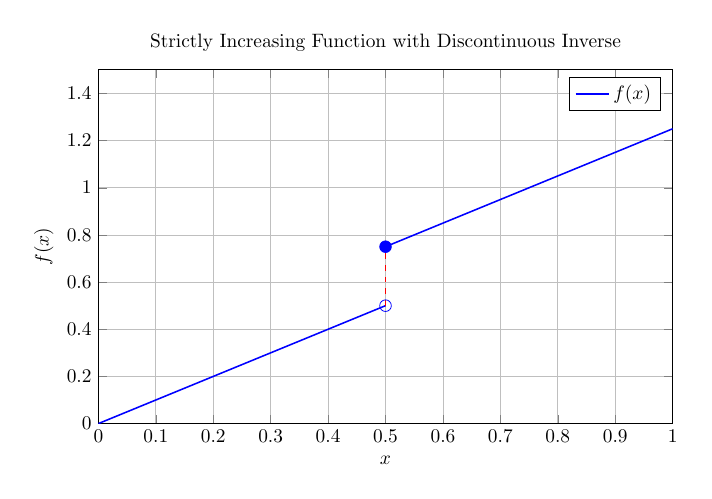
\begin{tikzpicture}[scale=0.7]
        \begin{axis}[
            width=12cm,
            height=8cm,
            xlabel={$x$},
            ylabel={$f(x)$},
            xmin=0, xmax=1,
            ymin=0, ymax=1.5,
            grid=major,
            title={Strictly Increasing Function with Discontinuous Inverse}
        ]
        
        % Plot the function f(x)
        \addplot[blue, thick] coordinates {(0,0) (0.5,0.5)};
        \addplot[blue, thick] coordinates {(0.5,0.75) (1,1.25)};
        \addplot[only marks, mark=*, mark size=3pt, blue] coordinates {(0.5,0.75)};
        \addplot[only marks, mark=o, mark size=3pt, blue] coordinates {(0.5,0.5)};
        \addlegendentry{$f(x)$}
        
        % Mark the jump
        \addplot[dashed, red] coordinates {(0.5,0.5) (0.5,0.75)};
        \end{axis}
    \end{tikzpicture}
    \caption{The function $f(x)$ is strictly increasing but has a jump discontinuity at $x=1/2$, creating a gap in the range that makes the inverse discontinuous.}
    \end{figure}
\bigskip\noindent\textbf{Solution:}
(a) For increasing $f$, right and left limits exist. The jumps on disjoint points add up and are bounded by the total variation $f(b-)-f(a+)$. A telescoping partition argument gives the inequality.

(b) For each $m\in\mathbb{N}$, the set of points where the jump $\ge 1/m$ is finite by (a). The discontinuity set is the countable union over $m$, hence countable.

(c) In any open subinterval, if all points were discontinuities, jumps would sum to infinity or violate (a). Therefore at least one point is a continuity point.\qed

\begin{problembox}[4.64: Strictly Increasing with Discontinuous Inverse]
\begin{problemstatement}
Give an example of a function $f$, defined and strictly increasing on a set $S$ in $\mathbb{R}$, such that $f^{-1}$ is not continuous on $f(S)$.
\end{problemstatement}
\end{problembox}

\noindent\textbf{Strategy:} Construct a piecewise function that is strictly increasing but has a jump discontinuity. The inverse will have a corresponding jump, making it discontinuous. Use a function that has different definitions on different intervals with a gap in the range.

\bigskip\noindent\textbf{Solution:}
Let $S=[0,1]$ and define
\[
f(x)=\begin{cases}
x,& x<\tfrac12,\\
\tfrac34,& x=\tfrac12,\\
x+\tfrac14,& x>\tfrac12.
\end{cases}
\]
Then $f$ is strictly increasing on $[0,1]$, but $f(S)=[0,\tfrac12)\cup\{\tfrac34\}\cup(\tfrac34,\tfrac54]$. The inverse $f^{-1}$ has a jump at $y=\tfrac34$ (approaching from below gives preimages $\to\tfrac12^-$, while at $\tfrac34$ the preimage is $\tfrac12$ and from above preimages $\to\tfrac12^+$), hence $f^{-1}$ is not continuous.

\qed

\begin{problembox}[4.65: Continuity of Strictly Increasing Functions]
\begin{problemstatement}
Let $f$ be strictly increasing on a subset $S$ of $\mathbb{R}$. Assume that the image $f(S)$ has one of the following properties: 
(a) $f(S)$ is open; (b) $f(S)$ is connected; (c) $f(S)$ is closed. Prove that $f$ must be continuous on $S$.
\end{problemstatement}
\end{problembox}

\noindent\textbf{Strategy:} Use the fact that strictly increasing functions can only have jump discontinuities. A jump at a point would create a gap in the image, which contradicts the given properties: (a) and (b) because gaps disconnect the image, (c) because a gap creates a limit point not in the image.

\bigskip\noindent\textbf{Solution:}
A strictly increasing function on $\mathbb{R}$ has only jump discontinuities. A jump at $x$ would create a gap in $f(S)$ (two-sided limits differ): this contradicts (a) and (b). Under (c), a jump would create a limit point of $f(S)$ not contained in $f(S)$, contradicting closedness. Hence no jumps; $f$ is continuous.\qed

\section{Metric spaces and fixed points}

\begin{definitionssection}{Definitions and Theorems}
\end{definitionssection}

\begin{definition}[Contraction Mapping]
A function $f: S \to S$ on a metric space $(S,d)$ is a contraction if there exists $\alpha \in [0,1)$ such that $d(f(x), f(y)) \leq \alpha d(x,y)$ for all $x,y \in S$.
\end{definition}

\noindent\begin{importance}
\textbf{Importance:}Contraction mappings are functions that "shrink" distances by a fixed factor less than 1. This property makes them essential for fixed point theory and iterative methods. They provide a powerful tool for proving existence and uniqueness of solutions to equations and for developing numerical algorithms.
\end{importance}\begin{theorem}[Contraction Mapping Theorem]
Let $(S,d)$ be a complete metric space and $f: S \to S$ a contraction. Then $f$ has a unique fixed point $p$, and for any $x \in S$, the sequence $f^n(x)$ converges to $p$.
\end{theorem}

\noindent\begin{importance}
\textbf{Importance:}This is one of the most important theorems in analysis, providing a powerful method for proving existence and uniqueness of solutions to equations. It guarantees that iterative methods converge to the unique solution and provides explicit error bounds. This theorem is the foundation for many numerical algorithms and existence proofs.
\end{importance}\begin{itemize}
\item Existence and uniqueness of solutions to equations
\item Numerical methods and iterative algorithms
\item Differential equations and boundary value problems
\item Functional analysis and operator theory
\item Optimization theory and algorithms
\end{itemize}

\begin{theorem}[Invariance of Domain]
If $f: \mathbb{R}^n \to \mathbb{R}^n$ is continuous and injective, then $f$ is open.
\end{theorem}

\noindent\begin{importance}
\textbf{Importance:}This is a deep result in topology that shows that continuous injective maps preserve the topological structure of Euclidean spaces. It's essential for understanding the behavior of continuous functions and is fundamental in differential topology and geometric analysis.
\end{importance}
\begin{problembox}[4.66: The Metric Space of Bounded Functions]
\begin{problemstatement}
Let $B(S)$ denote the set of all real-valued functions which are defined and bounded on a nonempty set $S$. If $f \in B(S)$, let $\|f\| = \sup_{x \in S} |f(x)|$. The number $\|f\|$ is called the "sup norm" of $f$.
\begin{enumerate}[label=(\alph*)]
\item Prove that the formula $d(f, g) = \|f - g\|$ defines a metric $d$ on $B(S)$.
\item Prove that the metric space $(B(S), d)$ is complete. 
\end{enumerate}
\textit{Hint.} If $(f_n)$ is a Cauchy sequence in $B(S)$, show that $\{f_n(x)\}$ is a Cauchy sequence of real numbers for each $x$ in $S$.
\end{problemstatement}
\end{problembox}

\noindent\textbf{Strategy:} For (a), verify the metric axioms using properties of the sup norm. For (b), use the hint to show that for each $x \in S$, the sequence $(f_n(x))$ is Cauchy in $\mathbb{R}$ and converges to some $f(x)$. Then show that the resulting function $f$ is bounded and that $f_n \to f$ in the sup norm.

\bigskip\noindent\textbf{Solution:}
(a) Nonnegativity, symmetry, and triangle inequality follow from properties of the sup norm; $\|f-g\|=0$ iff $f=g$.

(b) If $(f_n)$ is Cauchy in sup norm, then for each $x$, $(f_n(x))$ is Cauchy in $\mathbb{R}$ and converges to some $f(x)$. Uniform Cauchy-ness yields $\|f_n-f\|\to 0$, so $f\in B(S)$ and $f_n\to f$ in $d$.\qed

\begin{problembox}[4.67: The Metric Space of Continuous Bounded Functions]
\begin{problemstatement}
Refer to Exercise 4.66 and let $C(S)$ denote the subset of $B(S)$ consisting of all functions continuous and bounded on $S$, where now $S$ is a metric space.
\begin{enumerate}[label=(\alph*)]
\item Prove that $C(S)$ is a closed subset of $B(S)$.
\item Prove that the metric subspace $C(S)$ is complete.
\end{enumerate}
\end{problemstatement}
\end{problembox}

\noindent\textbf{Strategy:} For (a), use the fact that the uniform limit of continuous functions is continuous. For (b), use the result that closed subspaces of complete metric spaces are complete, or repeat the proof from Exercise 4.66 and use uniform convergence to preserve continuity.

\bigskip\noindent\textbf{Solution:}
(a) If $f_n\in C(S)$ and $\|f_n-f\|\to 0$, then $f$ is the uniform limit of continuous functions, hence continuous. Thus $f\in C(S)$; $C(S)$ is closed.

(b) Closed subspaces of complete metric spaces are complete. Alternatively, repeat the proof in 4.66 and use uniform convergence to pass continuity to the limit.\qed

\begin{problembox}[4.68: Application of the Fixed-Point Theorem]
\begin{problemstatement}
Refer to the proof of the fixed-point theorem (Theorem 4.48) for notation.
\begin{enumerate}[label=(\alph*)]
\item Prove that $d(p_n, p_{n+1}) \leq d(x, f(x)) \alpha^n / (1 - \alpha)$. This inequality, which is useful in numerical work, provides an estimate for the distance from $p_n$ to the fixed point $p$. An example is given in (b).
\item Take $f(x) = (x + 2/x)/2$, $S = [1, +\infty)$. Prove that $f$ is a contraction of $S$ with contraction constant $\alpha = 1/2$ and fixed point $p = \sqrt{2}$. Form the sequence $(p_n)$ starting with $x=p_0=1$ and show that $|p_n - \sqrt{2}| \le 2^{-n}$.
\end{enumerate}
\end{problemstatement}
\end{problembox}

\noindent\textbf{Strategy:} For (a), use the contraction property to bound the distance between consecutive iterates and sum the geometric series. For (b), show that $f$ is a contraction by analyzing its derivative, find the fixed point by solving $f(x) = x$, and apply the bound from (a).

% Plot showing the fixed point iteration
\begin{figure}[h!]
    \centering
    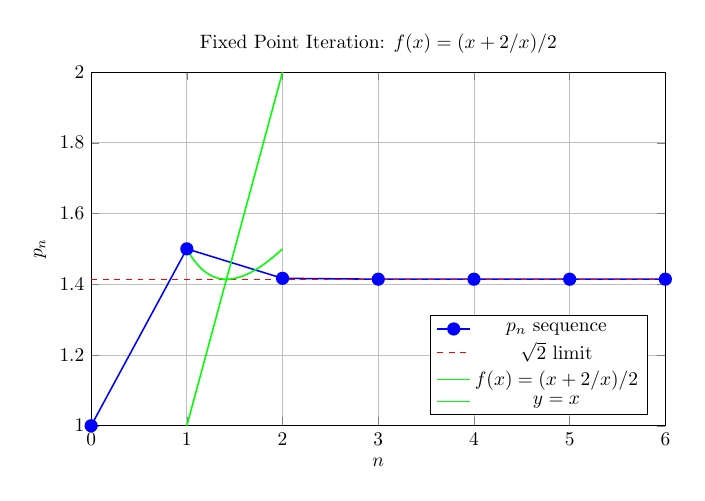
\begin{tikzpicture}[scale=0.7]
        \begin{axis}[
            width=12cm,
            height=8cm,
            xlabel={$n$},
            ylabel={$p_n$},
            xmin=0, xmax=6,
            ymin=1, ymax=2,
            grid=major,
            legend pos=south east,
            title={Fixed Point Iteration: $f(x) = (x + 2/x)/2$}
        ]
        
        % Plot the sequence
        \addplot[blue, thick, mark=*, mark size=3pt] coordinates {
            (0,1) (1,1.5) (2,1.416667) (3,1.414216) (4,1.414214) (5,1.414214) (6,1.414214)
        };
        \addlegendentry{$p_n$ sequence}
        
        % Horizontal line at sqrt(2)
        \addplot[dashed, red] coordinates {(0,1.414213562) (6,1.414213562)};
        \addlegendentry{$\sqrt{2}$ limit}
        
        % Plot the function f(x) = (x + 2/x)/2
        \addplot[green, thick, samples=100, domain=1:2] {(x + 2/x)/2};
        \addlegendentry{$f(x) = (x + 2/x)/2$}
        \addplot[green, thick, samples=100, domain=1:2] {x};
        \addlegendentry{$y = x$}
        \end{axis}
    \end{tikzpicture}
    \caption{The Babylonian method for computing $\sqrt{2}$: the sequence $p_n$ converges quadratically to $\sqrt{2} \approx 1.414213562$. The function $f(x) = (x + 2/x)/2$ has a fixed point at $x = \sqrt{2}$.}
    \end{figure}
    
\bigskip\noindent\textbf{Solution:}
(a) In a contraction with constant $\alpha\in(0,1)$, $d(p_{n+k},p_{n+k+1})\le \alpha^{n+k}d(x,f(x))$. Hence
\[
d(p_n,p)\le \sum_{k=0}^{\infty} d(p_{n+k},p_{n+k+1})\le d(x,f(x))\sum_{k=0}^{\infty}\alpha^{n+k}=\frac{\alpha^n}{1-\alpha}d(x,f(x)).
\]

(b) On $[1,\infty)$, $f'(x)=\tfrac12\big(1-\tfrac{2}{x^2}\big)$ so $|f'(x)|\le \tfrac12$, hence $f$ is a contraction with $\alpha=1/2$. Fixed points solve $x=\tfrac12(x+2/x)$, i.e., $x^2=2$, so $p=\sqrt2$. The bound in (a) gives $|p_n-\sqrt2|\le 2^{-n}|x-f(x)|\cdot\tfrac{1}{1-1/2}=2^{-n}\cdot 2|x-f(x)|$. With $x=p_0=1$, a direct induction using the mean value theorem or the quadratic convergence of the Babylonian method yields $|p_n-\sqrt2|\le 2^{-n}$.
\qed

\begin{problembox}[4.69: Necessity of Conditions for Fixed-Point Theorem]
\begin{problemstatement}
Show by counterexamples that the fixed-point theorem for contractions need not hold if either (a) the underlying metric space is not complete, or (b) the contraction constant $\alpha \ge 1$.
\end{problemstatement}
\end{problembox}

\noindent\textbf{Strategy:} For (a), use a non-complete metric space and a contraction whose fixed point lies outside the space. For (b), use functions that are Lipschitz with constant $\geq 1$ but have no fixed points, such as translations or dilations.

\bigskip\noindent\textbf{Solution:}
(a) Let $S=(0,1)$ with usual metric and $f(x)=x/2$. Then $f$ is a contraction with fixed point $0\notin S$; no fixed point in $S$.

(b) Take $S=\mathbb{R}$ and $f(x)=x+1$; Lipschitz constant $\alpha=1$ but no fixed point. Or $f(x)=2x$ with $\alpha=2$.\qed

\begin{problembox}[4.70: Generalized Fixed-Point Theorem]
\begin{problemstatement}
Let $f: S \to S$ be a function from a complete metric space $(S, d)$ into itself. Assume there is a real sequence $(a_n)$ which converges to $0$ such that $d(f^n(x), f^n(y)) \le a_n d(x, y)$ for all $n \ge 1$ and all $x, y$ in $S$, where $f^n$ is the $n$th iterate of $f$, that is, 

$f^1(x) = f(x)$, $f^{n+1}(x) = f(f^n(x))$, for $n \ge 1$. 

Prove that $f$ has a unique fixed point. \textit{Hint.} Apply the fixed-point theorem to $f^m$ for a suitable $m$.
\end{problemstatement}
\end{problembox}

\noindent\textbf{Strategy:} Use the hint to find a large enough $m$ such that $a_m < 1$, making $f^m$ a contraction. Apply the contraction mapping theorem to $f^m$ to find a unique fixed point $p$, then show that $f(p)$ is also a fixed point of $f^m$, hence $f(p) = p$.

\bigskip\noindent\textbf{Solution:}
Pick $m$ large so that $a_m<1$. Then $f^m$ is a contraction: $d(f^m(x),f^m(y))\le a_m d(x,y)$. By the contraction mapping theorem, $f^m$ has a unique fixed point $p$. Then $f(p)$ is also a fixed point of $f^m$, hence $f(p)=p$. Uniqueness for $f$ follows similarly.\qed

\begin{problembox}[4.71: Fixed Points for Distance-Shrinking Maps]
\begin{problemstatement}
Let $f: S \to S$ be a function from a metric space $(S, d)$ into itself such that
\[ d(f(x), f(y)) < d(x, y) \quad \text{whenever } x \neq y. \]
\begin{enumerate}[label=(\alph*)]
\item Prove that $f$ has at most one fixed point, and give an example of such an $f$ with no fixed point.
\item If $S$ is compact, prove that $f$ has exactly one fixed point. \textit{Hint.} Show that $g(x) = d(x, f(x))$ attains its minimum on $S$.
\item Give an example with $S$ compact in which $f$ is not a contraction.
\end{enumerate}
\end{problemstatement}
\end{problembox}

\noindent\textbf{Strategy:} For (a), use proof by contradiction: if there were two fixed points, their distance would be preserved, contradicting the shrinking property. For (b), use the hint and compactness to find a minimum of $g(x) = d(x, f(x))$, then show this minimum must be zero. For (c), find a function that shrinks distances but is not Lipschitz with constant $< 1$.

\bigskip\noindent\textbf{Solution:}
(a) If $f(x)=x$ and $f(y)=y$ with $x\ne y$, then $d(x,y)=d(f(x),f(y))<d(x,y)$, impossible. Example without a fixed point: $S=\mathbb{R}$, $f(x)=x+1$.

(b) On compact $S$, $g(x)=d(x,f(x))$ attains a minimum at $p$. If $g(p)>0$, then $g(f(p))=d(f(p),f^2(p))<d(p,f(p))=g(p)$, contradiction. Hence $g(p)=0$ and $p$ is a fixed point. Uniqueness holds by (a).

(c) Take $S=[0,1]$ and $f(x)=\sqrt{x}$. Then $d(f(x),f(y))<d(x,y)$ for $x\ne y$, but $f$ is not Lipschitz with constant $<1$ on $[0,1]$.\qed

\begin{problembox}[4.72: Iterated Function Systems]
\begin{problemstatement}
Assume that $f$ satisfies the condition in Exercise 4.71. If $x \in S$, let $p_0 = x$, $p_{n+1} = f(p_n)$, and $c_n = d(p_n, p_{n+1})$ for $n \geq 0$.
\begin{enumerate}[label=(\alph*)]
\item Prove that $\{c_n\}$ is a decreasing sequence, and let $c = \lim c_n$.
\item Assume there is a subsequence $\{p_{k(n)}\}$ which converges to a point $q$ in $S$. Prove that
\[c = d(q, f(q)) = d(f(q), f[f(q)])].\]
Deduce that $q$ is a fixed point of $f$ and that $p_n \to q$.
\end{enumerate}
\end{problemstatement}
\end{problembox}

\noindent\textbf{Strategy:} For (a), use the shrinking property to show that each $c_{n+1} < c_n$, making the sequence decreasing and convergent. For (b), use continuity of $f$ and the shrinking property to show that if $q$ is not a fixed point, then $d(f(q), f(f(q))) < d(q, f(q))$, contradicting the definition of $c$.

\bigskip\noindent\textbf{Solution:}
(a) By the shrinking property,
\[
c_{n+1}=d(p_{n+1},p_{n+2})=d(f(p_n),f(p_{n+1}))<d(p_n,p_{n+1})=c_n,
\]
so $(c_n)$ is strictly decreasing and converges to some $c\ge 0$.

(b) If $p_{k(n)}\to q$, then $p_{k(n)+1}=f(p_{k(n)})\to f(q)$ by continuity of $f$ (which follows from the shrinking property). Hence
\[
c=\lim c_{k(n)}=\lim d(p_{k(n)},p_{k(n)+1})=d(q,f(q)),
\]
and similarly $c=\lim c_{k(n)+1}=d(f(q),f(f(q)))$. Applying the shrinking property to $q$ and $f(q)$ yields $d(f(q),f(f(q)))<d(q,f(q))$ unless $q=f(q)$. Therefore $c=0$ and $q$ is a fixed point. Then $c_n\to 0$ and $(p_n)$ is Cauchy; in a compact (or complete with suitable conditions) space it converges to $q$.\qed

\begin{techniquessection}[Solving and Proving Techniques]

This chapter covers a wide range of analyzing limits, continuity, and convergence in various mathematical contexts. Here's a systematic the key proving strategies used throughout:

\subsection*{Proving Limits Exist}

\begin{itemize}
\item \textbf{Sequential Characterization:} To prove $\lim_{x \to a} f(x) = L$, show that for every sequence $(x_n) \to a$, we have $f(x_n) \to L$.

\item \textbf{$\varepsilon$-$\delta$ Definition:} For every $\varepsilon > 0$, find a $\delta > 0$ such that $|x - a| < \delta$ implies $|f(x) - L| < \varepsilon$.

\item \textbf{Squeeze Theorem:} If $g(x) \leq f(x) \leq h(x)$ near $a$ and $\lim_{x \to a} g(x) = \lim_{x \to a} h(x) = L$, then $\lim_{x \to a} f(x) = L$.

\item \textbf{Algebraic Manipulation:} Use techniques like rationalization, factoring, or Taylor expansions to simplify expressions before taking limits.
\end{itemize}

\subsection*{Proving Convergence of Sequences}

\begin{itemize}
\item \textbf{Monotone Convergence:} Show the sequence is bounded and monotone (increasing or decreasing).

\item \textbf{Cauchy Criterion:} Prove the sequence is Cauchy by showing $|x_n - x_m| < \varepsilon$ for all $n, m \geq N$.

\item \textbf{Comparison with Known Sequences:} Compare with geometric sequences, use ratio tests, or compare with sequences with known limits.

\item \textbf{Recursive Analysis:} For recursive sequences, find the fixed point by solving $x = f(x)$, then show convergence to this fixed point.
\end{itemize}

\subsection*{Proving Continuity}

\begin{itemize}
\item \textbf{Sequential Continuity:} Show that if $x_n \to x$, then $f(x_n) \to f(x)$.

\item \textbf{$\varepsilon$-$\delta$ Definition:} For every $\varepsilon > 0$, find $\delta > 0$ such that $|x - y| < \delta$ implies $|f(x) - f(y)| < \varepsilon$.

\item \textbf{Composition of Continuous Functions:} Use the fact that compositions, sums, products, and quotients of continuous functions are continuous.

\item \textbf{Preimage Characterization:} Show that preimages of open sets are open (or preimages of closed sets are closed).
\end{itemize}

\subsection*{Proving Uniform Continuity}

\begin{itemize}
\item \textbf{Direct Verification:} Find a $\delta$ that works for all points simultaneously.

\item \textbf{Lipschitz Condition:} Show $|f(x) - f(y)| \leq M|x - y|$ for some constant $M$.

\item \textbf{Compact Domain:} On compact sets, continuity implies uniform continuity.

\item \textbf{Extension to Closure:} Extend uniformly continuous functions to the closure of their domain.
\end{itemize}

\subsection*{Proving Connectedness}

\begin{itemize}
\item \textbf{Path-Connectedness:} Show that any two points can be joined by a continuous path.

\item \textbf{Contradiction Method:} Assume disconnectedness and derive a contradiction.

\item \textbf{Intermediate Value Property:} Use the fact that continuous functions preserve connectedness.

\item \textbf{Closure Properties:} Show that the closure of a connected set is connected.
\end{itemize}

\subsection*{Proving Compactness}

\begin{itemize}
\item \textbf{Sequential Compactness:} Show that every sequence has a convergent subsequence.

\item \textbf{Heine-Borel (in $\mathbb{R}^n$):} Show the set is closed and bounded.

\item \textbf{Finite Subcover:} Show that every open cover has a finite subcover.

\item \textbf{Continuous Image:} Show the set is the continuous image of a compact set.
\end{itemize}

\subsection*{Proving Fixed Points}

\begin{itemize}
\item \textbf{Contraction Mapping:} Show the function is a contraction and apply the contraction mapping theorem.

\item \textbf{Iteration Method:} Start with any point and show the sequence of iterates converges.

\item \textbf{Compactness + Distance Shrinking:} On compact spaces, show $d(f(x), f(y)) < d(x,y)$ for $x \neq y$.

\item \textbf{Banach Fixed Point:} Use the complete metric space version of the contraction mapping theorem.
\end{itemize}

\subsection*{Proving Discontinuity}

\begin{itemize}
\item \textbf{Sequential Method:} Find two sequences converging to the same point but with different function value limits.

\item \textbf{Oscillation:} Show the oscillation at a point is positive.

\item \textbf{One-Sided Limits:} Show that left and right limits exist but are different (jump discontinuity).

\item \textbf{Path Dependence:} For functions of several variables, show the limit depends on the path taken.
\end{itemize}

\subsection*{Proving Completeness}

\begin{itemize}
\item \textbf{Cauchy Sequences:} Show that every Cauchy sequence converges to a point in the space.

\item \textbf{Nested Closed Sets:} Use Cantor's intersection theorem with nested closed sets of decreasing diameter.

\item \textbf{Isometric Embedding:} Embed the space into a complete space and show the embedding is onto.

\item \textbf{Contraction Mapping:} Use the fact that complete spaces are preserved under contractions.
\end{itemize}

\subsection*{Common Patterns and Strategies}

\begin{itemize}
\item \textbf{Proof by Contradiction:} Assume the opposite and derive a contradiction.

\item \textbf{Induction:} Use mathematical induction for recursive sequences or properties that hold for all natural numbers.

\item \textbf{Approximation:} Approximate complicated objects with simpler ones (e.g., rationals approximating reals).

\item \textbf{Partitioning:} Break complex problems into simpler cases or use the trichotomy property.

\item \textbf{Uniformity:} When local properties hold everywhere, they often become uniform properties.
\end{itemize}

\section{Chapter Summary: Key Relationships and Implications}

This section summarizes the fundamental relationships and implications established throughout Chapter 4, showing how different concepts connect and build upon each other.

\subsection*{Sequences and Convergence}

\begin{itemize}
\item \textbf{Cauchy sequence} $\rightarrow$ \textbf{convergent sequence} (in complete metric spaces)
\item \textbf{Bounded monotone sequence} $\rightarrow$ \textbf{convergent sequence}
\item \textbf{Convergent sequence} $\rightarrow$ \textbf{Cauchy sequence}
\item \textbf{Subsequence of convergent sequence} $\rightarrow$ \textbf{converges to same limit}
\item \textbf{Geometric sequence with $|z| < 1$} $\rightarrow$ \textbf{converges to 0}
\item \textbf{Geometric sequence with $|z| > 1$} $\rightarrow$ \textbf{diverges}
\end{itemize}

\subsection*{Continuity Relationships}

\begin{itemize}
\item \textbf{Uniformly continuous function} $\rightarrow$ \textbf{continuous function}
\item \textbf{Continuous function on compact set} $\rightarrow$ \textbf{uniformly continuous function}
\item \textbf{Continuous function} $\rightarrow$ \textbf{sequentially continuous function}
\item \textbf{Sequentially continuous function} $\rightarrow$ \textbf{continuous function} (in metric spaces)
\item \textbf{Additive function continuous at one point} $\rightarrow$ \textbf{continuous everywhere}
\item \textbf{Continuous function} $\rightarrow$ \textbf{preserves connectedness}
\item \textbf{Continuous function} $\rightarrow$ \textbf{preserves compactness}
\item \textbf{Continuous function on compact set} $\rightarrow$ \textbf{attains maximum and minimum}
\item \textbf{Continuous function on interval} $\rightarrow$ \textbf{has intermediate value property}
\item \textbf{One-to-one continuous function on interval} $\rightarrow$ \textbf{strictly monotonic}
\end{itemize}

\subsection*{Metric Space Properties}

\begin{itemize}
\item \textbf{Compact metric space} $\rightarrow$ \textbf{every sequence has convergent subsequence}
\item \textbf{Compact metric space} $\rightarrow$ \textbf{complete metric space}
\item \textbf{Complete metric space} $\rightarrow$ \textbf{closed subset is complete}
\item \textbf{Closed subset of complete space} $\rightarrow$ \textbf{complete subset}
\item \textbf{Compact subset of $\mathbb{R}^n$} $\rightarrow$ \textbf{closed and bounded}
\item \textbf{Closed and bounded subset of $\mathbb{R}^n$} $\rightarrow$ \textbf{compact subset}
\item \textbf{Connected metric space} $\rightarrow$ \textbf{only clopen subsets are empty set and whole space}
\item \textbf{Disconnected metric space} $\rightarrow$ \textbf{has nonempty proper clopen subset}
\end{itemize}

\subsection*{Function Properties}

\begin{itemize}
\item \textbf{Uniformly continuous function} $\rightarrow$ \textbf{preserves Cauchy sequences}
\item \textbf{Continuous function} $\rightarrow$ \textbf{does not necessarily preserve Cauchy sequences}
\item \textbf{Strictly increasing function} $\rightarrow$ \textbf{has countable discontinuities}
\item \textbf{Monotonic function} $\rightarrow$ \textbf{has one-sided limits at every point}
\item \textbf{Convex subset} $\rightarrow$ \textbf{connected subset}
\item \textbf{Path-connected space} $\rightarrow$ \textbf{connected space}
\item \textbf{Connected space} $\rightarrow$ \textbf{does not necessarily imply path-connected}
\end{itemize}

\subsection*{Fixed Point Theory}

\begin{itemize}
\item \textbf{Contraction mapping on complete metric space} $\rightarrow$ \textbf{has unique fixed point}
\item \textbf{Distance-shrinking function on compact space} $\rightarrow$ \textbf{has unique fixed point}
\item \textbf{Contraction mapping} $\rightarrow$ \textbf{iterates converge to fixed point}
\item \textbf{Non-contraction function} $\rightarrow$ \textbf{may not have fixed points}
\item \textbf{Incomplete metric space} $\rightarrow$ \textbf{contraction may not have fixed point}
\end{itemize}

\subsection*{Limits and Discontinuities}

\begin{itemize}
\item \textbf{Two-dimensional limit exists} $\rightarrow$ \textbf{iterated limits exist and are equal}
\item \textbf{Iterated limits exist and are equal} $\rightarrow$ \textbf{does not necessarily imply two-dimensional limit exists}
\item \textbf{Function continuous in each variable} $\rightarrow$ \textbf{does not necessarily imply multi-variable continuity}
\item \textbf{Multi-variable continuous function} $\rightarrow$ \textbf{continuous in each variable}
\item \textbf{Removable discontinuity} $\rightarrow$ \textbf{limit exists but differs from function value}
\item \textbf{Jump discontinuity} $\rightarrow$ \textbf{one-sided limits exist but are different}
\item \textbf{Essential discontinuity} $\rightarrow$ \textbf{at least one one-sided limit does not exist}
\end{itemize}

\subsection*{Special Functions and Properties}

\begin{itemize}
\item \textbf{Additive function + continuity at one point} $\rightarrow$ \textbf{linear function $f(x) = ax$}
\item \textbf{Function zero on rationals + continuity} $\rightarrow$ \textbf{function zero everywhere}
\item \textbf{Function continuous on rationals + discontinuous on irrationals} $\rightarrow$ \textbf{nowhere continuous}
\item \textbf{Function with exactly two preimages for every value} $\rightarrow$ \textbf{necessarily discontinuous}
\item \textbf{Space-filling curve} $\rightarrow$ \textbf{cannot be one-to-one}
\item \textbf{Homeomorphism} $\rightarrow$ \textbf{preserves topological properties but not metric properties}
\end{itemize}

\subsection*{Topological Invariants}

\begin{itemize}
\item \textbf{Connectedness} $\rightarrow$ \textbf{topological invariant (preserved by homeomorphisms)}
\item \textbf{Compactness} $\rightarrow$ \textbf{topological invariant}
\item \textbf{Completeness} $\rightarrow$ \textbf{not a topological invariant}
\item \textbf{Boundedness} $\rightarrow$ \textbf{not a topological invariant}
\item \textbf{Openness} $\rightarrow$ \textbf{topological invariant}
\item \textbf{Closedness} $\rightarrow$ \textbf{topological invariant}
\end{itemize}

\subsection*{Practical Implications}

\begin{itemize}
\item \textbf{Uniform continuity} $\rightarrow$ \textbf{enables extension to closure}
\item \textbf{Compactness} $\rightarrow$ \textbf{enables uniform continuity from continuity}
\item \textbf{Connectedness} $\rightarrow$ \textbf{enables intermediate value theorem}
\item \textbf{Completeness} $\rightarrow$ \textbf{enables contraction mapping theorem}
\item \textbf{Density of rationals} $\rightarrow$ \textbf{enables approximation techniques}
\item \textbf{Sequential characterization} $\rightarrow$ \textbf{enables limit proofs via sequences}
\end{itemize}

\medskip

\noindent\textbf{Key Insight:} These relationships form the foundation of modern analysis, showing how different mathematical concepts interconnect and support each other. Understanding these implications is crucial for developing intuition about which properties imply others and for constructing proofs that build upon established results.
\end{techniquessection}
